%%%%%%%%%%%%%%%%%%%%%%%%%%%%%%%%%%%%%%%%%%%%%%%%%%%%%%%%%%%%%%%%%%%%%%%%%%%%%%%%
%% Plantilla de memoria en LaTeX para la ETSIT - Universidad Rey Juan Carlos
%%
%% Por Gregorio Robles <grex arroba gsyc.urjc.es>
%%     Grupo de Sistemas y Comunicaciones
%%     Escuela Técnica Superior de Ingenieros de Telecomunicación
%%     Universidad Rey Juan Carlos
%% (muchas ideas tomadas de Internet, colegas del GSyC, antiguos alumnos...
%%  etc. Muchas gracias a todos)
%%
%% La última versión de esta plantilla está siempre disponible en:
%%     https://github.com/gregoriorobles/plantilla-memoria
%%
%% Para obtener PDF, ejecuta en la shell:
%%   make
%% (las imágenes deben ir en PNG o JPG)

%%%%%%%%%%%%%%%%%%%%%%%%%%%%%%%%%%%%%%%%%%%%%%%%%%%%%%%%%%%%%%%%%%%%%%%%%%%%%%%%

\documentclass[a4paper, 12pt]{book}
%\usepackage[T1]{fontenc}
\usepackage[a4paper, left=2.5cm, right=2.5cm, top=3cm, bottom=3cm]{geometry}
\usepackage{times}
\usepackage[utf8]{inputenc}
\usepackage[spanish]{babel} % Comenta esta línea si tu memoria es en inglés
\usepackage{url}
%\usepackage[dvipdfm]{graphicx}
\usepackage{graphicx}
\usepackage{float}  %% H para posicionar figuras
\usepackage[nottoc, notlot, notlof, notindex]{tocbibind} %% Opciones de índice
\usepackage{latexsym}  %% Logo LaTeX
\usepackage{listings}
\usepackage{color}
\usepackage{xcolor}
\lstdefinestyle{consola} {
   numbers=none,
   backgroundcolor=\color{black},
   basicstyle=\small\bf\ttfamily\color{white}
}

\colorlet{punct}{red!60!black}
\definecolor{background}{HTML}{EEEEEE}
\definecolor{delim}{RGB}{20,105,176}
\colorlet{numb}{magenta!60!black}

\lstdefinelanguage{json}{
    basicstyle=\normalfont\ttfamily,
    showstringspaces=false,
    breaklines=true,
    literate=
     *{0}{{{\color{numb}0}}}{1}
      {1}{{{\color{numb}1}}}{1}
      {2}{{{\color{numb}2}}}{1}
      {3}{{{\color{numb}3}}}{1}
      {4}{{{\color{numb}4}}}{1}
      {5}{{{\color{numb}5}}}{1}
      {6}{{{\color{numb}6}}}{1}
      {7}{{{\color{numb}7}}}{1}
      {8}{{{\color{numb}8}}}{1}
      {9}{{{\color{numb}9}}}{1}
      {:}{{{\color{punct}{:}}}}{1}
      {,}{{{\color{punct}{,}}}}{1}
      {\{}{{{\color{delim}{\{}}}}{1}
      {\}}{{{\color{delim}{\}}}}}{1}
      {[}{{{\color{delim}{[}}}}{1}
      {]}{{{\color{delim}{]}}}}{1},
}


\title{Análisis de clonado y abstracción en Scratch}
\author{Felipe Enmanuel Sandoval Sibada}

\renewcommand{\baselinestretch}{1.5}  %% Interlineado

\begin{document}

\renewcommand{\refname}{Bibliografía}  %% Renombrando
\renewcommand{\appendixname}{Apéndice}

%%%%%%%%%%%%%%%%%%%%%%%%%%%%%%%%%%%%%%%%%%%%%%%%%%%%%%%%%%%%%%%%%%%%%%%%%%%%%%%%
% PORTADA

\begin{titlepage}
\begin{center}

\includegraphics[scale=0.6]{img/logo_vect.png}
\Large

\vspace{1.75cm}

\Large
GRADO EN INGENIERÍA EN SISTEMAS AUDIOVISUALES Y MULTIMEDIA

\vspace{0.4cm}

\large
Curso Académico 2021/2022

\vspace{0.8cm}

Trabajo Fin de Grado

\vspace{2.0cm}

\LARGE
ANÁLISIS DE CLONADO Y ABSTRACCIÓN EN SCRATCH

\vspace{4cm}

\large
Autor : Felipe Enmanuel Sandoval Sibada \\
Tutor : Dr. Gregorio Robles
\end{center}
\end{titlepage}

\newpage
\mbox{}
\thispagestyle{empty} % para que no se numere esta pagina


%%%%%%%%%%%%%%%%%%%%%%%%%%%%%%%%%%%%%%%%%%%%%%%%%%%%%%%%%%%%%%%%%%%%%%%%%%%%%%%%
%%%% Para firmar
\clearpage
\pagenumbering{gobble}
\chapter*{}

\vspace{-4cm}
\begin{center}
\LARGE
\textbf{Trabajo Fin de Grado}

\vspace{1cm}
\large
Análisis de Clonado y Abstracción en Scratch

\vspace{1cm}
\large
\textbf{Autor :} Felipe Enmanuel Sandoval Sibada \\
\textbf{Tutor :} Dr. Gregorio Robles

\end{center}

\vspace{1cm}
La defensa del presente Proyecto Fin de Carrera se realizó el día \qquad$\;\,$ de \qquad\qquad\qquad\qquad \newline de 2022, siendo calificada por el siguiente tribunal:


\vspace{0.5cm}
\textbf{Presidente:}

\vspace{1.2cm}
\textbf{Secretario:}

\vspace{1.2cm}
\textbf{Vocal:}



\vspace{1.2cm}
y habiendo obtenido la siguiente calificación:

\vspace{1cm}
\textbf{Calificación:}


\vspace{1cm}
\begin{flushright}
Fuenlabrada, a \qquad$\;\,$ de \qquad\qquad\qquad\qquad de 2022
\end{flushright}

%%%%%%%%%%%%%%%%%%%%%%%%%%%%%%%%%%%%%%%%%%%%%%%%%%%%%%%%%%%%%%%%%%%%%%%%%%%%%%%%
%%%% Dedicatoria

\chapter*{}
\pagenumbering{Roman} % para comenzar la numeracion de paginas en numeros romanos
\begin{flushright}
\textit{Dedicado a \\
mi madre, por su apoyo incondicional.}
\end{flushright}

%%%%%%%%%%%%%%%%%%%%%%%%%%%%%%%%%%%%%%%%%%%%%%%%%%%%%%%%%%%%%%%%%%%%%%%%%%%%%%%%
%%%% Agradecimientos

\chapter*{Agradecimientos}
%\addcontentsline{toc}{chapter}{Agradecimientos} % si queremos que aparezca en el índice
\markboth{AGRADECIMIENTOS}{AGRADECIMIENTOS} % encabezado 
No ha sido fácil...\\

Salir de mi zona de confort ha sido una de las decisiones más difíciles y, a la vez, gratificantes que he tomado en mi vida. En el año 2014 decidí embarcarme hacía una de las mejores ciudades en las que he podido vivir, mi querida Madrid. Evidentemente no ha sido fácil dejar atrás a familiares, amigos, costumbres y un largo etcétera, pero cambiar de rutina hizo que me volviese una persona independiente, curiosa y resiliente. 

Quiero agradecer a mis padres por su apoyo, comprensión, entendimiento y soporte. A mi madre, Flor Marjorie, por siempre estar ahí en cada momento, gracias a ti me convertí en la persona que soy hoy en día. No son suficientes las palabras para expresar mi gratitud, te quiero un mundo. 

Gracias a ti, Nathalie, por escucharme y entenderme, por tu paciencia en momentos difíciles, por ayudarme a desconectar y por nunca dejar que tirase la toalla. Me demuestras que la motivación es importante pero que sin disciplina y sin hábitos de estudio, de poco vale. Estoy seguro que el futuro nos deparará momentos y vivencias memorables que podremos compartir. Te adoro.

A mis amigos, gracias por su comprensión y por seguir contando conmigo para todos los planes. Son incontables las experiencias vividas y los \textit{``tours''} que hicimos en casi todas las bibliotecas de Madrid. Gracias por enseñarme que en equipo la universidad es más fácil.

Por último quiero agradecer a mi tutor, Gregorio, por brindarme la oportunidad de trabajar junto a él y demostrarme que la enseñanza es un tema de vocación. Con este proyecto he ratificado la importancia de motivar y dotar de herramientas a las generaciones más jóvenes, ya que solo así será posible desarrollar su potencial profesional y humano. Muchas gracias por tu paciencia, amabilidad y tiempo, especialmente porque, a pesar de haber atravesado una pandemia mundial, al final hemos logrado salir adelante con este proyecto.

He sufrido y disfrutado con la experiencia universitaria, conocí personas muy especiales durante esta etapa que han y siguen siendo muy importantes en mi vida. 

Gracias a este viaje cuento con una caja de herramientas que me permitirán ejercer y desarrollarme en el apasionante oficio de la ingeniería y el mundo de las TIC.
A cualquiera que lea este proyecto, ¡Muchas Gracias!
\\\\
Y sí, no ha sido fácil... pero volvería a repetirlo.\\

%%%%%%%%%%%%%%%%%%%%%%%%%%%%%%%%%%%%%%%%%%%%%%%%%%%%%%%%%%%%%%%%%%%%%%%%%%%%%%%%
%%%% Resumen
\chapter*{Resumen}
%\addcontentsline{toc}{chapter}{Resumen} % si queremos que aparezca en el índice
\markboth{RESUMEN}{RESUMEN} % encabezado

En este trabajo se busca desarrollar una herramienta capaz de extraer y detectar duplicidad de código en proyectos de Scratch. Durante el proceso, se analizan los distintos bloques que conforman cada proyecto y se obtiene como resultado una lista con los conjuntos que mayor duplicidad presenten. Para lograr este objetivo se realiza un estudio estadístico tanto a nivel \textit{intra-sprite} como a nivel \textit{project-wide} haciendo uso del algoritmo de clustering de propagación por afinidad.

Esta idea surge a partir de otras herramientas que evalúan aspectos del pensamiento computacional, el cual abarca habilidades como el racionamiento lógico, la sincronización, el paralelismo, la representación de la información y la abstracción. Es el impacto de la duplicidad en esta última habilidad la que motiva la ejecución de este trabajo.

La herramienta se desarrolla usando Python como principal tecnología. Durante el trabajo se realizarán tests unitarios y guías de estilo para mejorar la calidad del código. Por último, se explicarán los resultados y analizarán, concluyendo si se consiguen o no, los objetivos planteados.


%referencia https://www.um.es/ead/red/46/moreno_robles_es.pdf

%%%%%%%%%%%%%%%%%%%%%%%%%%%%%%%%%%%%%%%%%%%%%%%%%%%%%%%%%%%%%%%%%%%%%%%%%%%%%%%%
%%%% Summary
\chapter*{Summary}
%\addcontentsline{toc}{chapter}{Summary}
\markboth{SUMMARY}{SUMMARY} % encabezado

This work aims to develop a tool capable of extracting and detecting code duplicity in Scratch projects. The different blocks that make up each project are analyzed to obtain a list of the most duplicated ones. In order to achieve this, a statistical study is carried out at both \textit{intra-sprite} and \textit{project-wide} levels, using the affinity propagation clustering algorithm.

The project idea arises from other tools that evaluate aspects such as computational thinking, which encompasses skills like logical reasoning, synchronization, parallelism, information representation, and abstraction. Impact of duplication on the last ability motivates the execution of this work.

The tool is developed using Python as the main technology. Through the work, unit tests and style guides are carried to improve the code quality. At last, results will be explained and analyzed, concluding whether or not the objectives are achieved.

%%%%%%%%%%%%%%%%%%%%%%%%%%%%%%%%%%%%%%%%%%%%%%%%%%%%%%%%%%%%%%%%%%%%%%%%%%%%%%%%
%%%%%%%%%%%%%%%%%%%%%%%%%%%%%%%%%%%%%%%%%%%%%%%%%%%%%%%%%%%%%%%%%%%%%%%%%%%%%%%%
% ÍNDICES %
%%%%%%%%%%%%%%%%%%%%%%%%%%%%%%%%%%%%%%%%%%%%%%%%%%%%%%%%%%%%%%%%%%%%%%%%%%%%%%%%

% Las buenas noticias es que los índices se generan automáticamente.
% Lo único que tienes que hacer es elegir cuáles quieren que se generen,
% y comentar/descomentar esa instrucción de LaTeX.

%%%% Índice de contenidos
\tableofcontents 
%%%% Índice de figuras
\cleardoublepage
%\addcontentsline{toc}{chapter}{Lista de figuras} % para que aparezca en el indice de contenidos
\listoffigures % indice de figuras
%%%% Índice de tablas
%\cleardoublepage
%\addcontentsline{toc}{chapter}{Lista de tablas} % para que aparezca en el indice de contenidos
%\listoftables % indice de tablas


%%%%%%%%%%%%%%%%%%%%%%%%%%%%%%%%%%%%%%%%%%%%%%%%%%%%%%%%%%%%%%%%%%%%%%%%%%%%%%%%
%%%%%%%%%%%%%%%%%%%%%%%%%%%%%%%%%%%%%%%%%%%%%%%%%%%%%%%%%%%%%%%%%%%%%%%%%%%%%%%%
% INTRODUCCIÓN %
%%%%%%%%%%%%%%%%%%%%%%%%%%%%%%%%%%%%%%%%%%%%%%%%%%%%%%%%%%%%%%%%%%%%%%%%%%%%%%%%

\cleardoublepage
\chapter{Introducción}
\label{sec:intro} % etiqueta para poder referenciar luego en el texto con ~\ref{sec:intro}
\pagenumbering{arabic} % para empezar la numeración de página con números

%En este capítulo se introduce el proyecto.
%Debería tener información general sobre el mismo, dando la información sobre el contexto en el que se ha %desarrollado.

%No te olvides de echarle un ojo a la página con los cinco errores de escritura más frecuentes\footnote{\url{http://www.tallerdeescritores.com/errores-de-escritura-frecuentes}}.

En este trabajo se busca crear una herramienta que, a partir del análisis de bloques de código en Scratch, pueda dar una visión general sobre la duplicidad de código en un proyecto. Se entenderá por duplicidad de código aquellos bloques que se repitan tanto a nivel \textit{intra-sprite} como \textit{project-wide}, considerando que los baremos de penalización son distintos según cada caso. Esto es así por consecuencia de los límites de la propia aplicación que restringe la re-utilización de código entre objetos de forma eficiente.

Antes que nada, es importante explicar una serie de conceptos del glosario de Scratch\footnote{\url{https://en.scratch-wiki.info/wiki}}. 

%FIXME: yo aquí añadiría una figura para cada concpeto.

\begin{itemize}
 \item Un bloque o \textit{block} es una pieza de código que ejecuta una acción. A nivel visual en la interfaz de Scratch, tienen formas de pieza de puzle con distintos colores y funcionalidades. En la imagen \ref{fig:blocks} se pueden apreciar varias estructuras de bloques. Más adelante se detallan los distintos tipos de bloques y las consideraciones especiales a tener en cuenta. 
 \item Un \textit{sprite} son los objetos de mi proyecto. A nivel visual, un sprite puede ser el fondo de tu escenario o una imagen, a modo de personaje. En la imagen \ref{fig:scratchsprite} se puede apreciar un ejemplo de un \textit{sprite}.
 \item Una función o \textit{script} es una colección de bloques. Su orden no es trivial, ya que determina cómo interactúan los \textit{sprites} entre sí, con el escenario y con el usuario. A nivel visual es una pila de varias piezas de puzle agrupadas.
 \item Un bloque personalizado o \textit{custom block} son las funciones definidas por el usuario. Este tipo de bloques permite crear funciones sin pensar en los tipos de bloques que contiene, por eso constituye una de las principales muestras de abstracción presentes en Scratch. También ayudan a reducir el tamaño de bloques del proyecto, ya que si un usuario tiene una larga cadena de código que sabe que usará mucho, tiene sentido usar un bloque personalizado. De esta manera, no se tiene que repetir código varias veces~\cite{scratchWeb}. En la imagen \ref{fig:script} se puede apreciar un \textit{custom block}, caracterizados por su color rosa, y un \textit{script}.
\end{itemize}.

\begin{figure}[htb!]
	\centering
    
\includegraphics[width=7cm, keepaspectratio]{img/blocks.jpg}
    \caption{Estructura de varios bloques y sus distintas formas}
    \label{fig:blocks}
\end{figure} 
 
\begin{figure}[htb!]
	\centering
    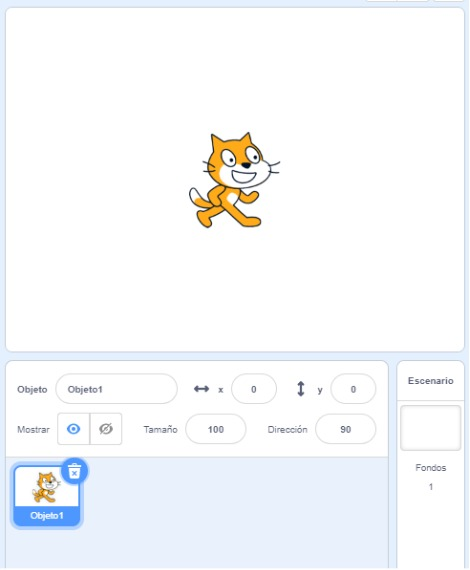
\includegraphics[width=8cm, keepaspectratio]{img/scratchsprite.jpg}
    \caption{Ejemplo de un sprite u objeto}
    \label{fig:scratchsprite}
\end{figure}

Para poder analizar la duplicidad de bloques de código en Scratch es necesario extraer la información del proyecto. Todos los datos de variables, objetos y bloques están contenidos en el fichero JSON dentro de la extensión \emph{.sb3} que usa Scratch. Una vez se obtiene esta información es necesario procesar, según una serie de parámetros, los bloques que más se repiten. Luego, el análisis de dichos datos se realiza mediante la asignación de familias de grupos entre puntos de datos, mejor conocido como algoritmo de propagación por afinidad. Se emplea este algoritmo ya que considera cada punto de datos como un nodo en una red que recursivamente itera hasta tener un buen conjunto de ejemplares para clasificar grupos~\cite{clusteringpaper}.

\begin{figure}[htb!]
	\centering
    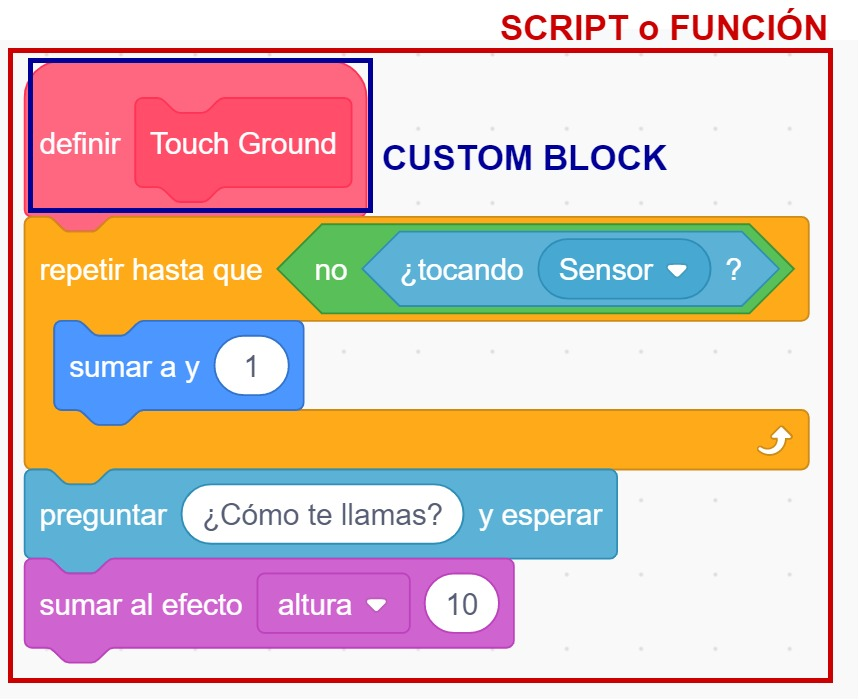
\includegraphics[width=9cm, keepaspectratio]{img/script.jpg}
    \caption{Ejemplo de un script y un custom block}
    \label{fig:script}
\end{figure}

\section{Contexto Personal}
\label{sec:contexto}

Como alumno del Grado de Ingeniería en Sistemas Audiovisuales y Multimedia (GISAM) he adquirido distintas competencias durante los años de carrera. Las asignaturas de programación son las que mayor interés suscitaron en mí. Después de unos años en los que por motivos profesionales me alejé de este campo, se me presentó la oportunidad de desarrollar una herramienta de software libre enfocado en aplicaciones de carácter pedagógico. La propuesta suponía un interesante reto que decidí afrontar. 

\section{Motivación}
\label{sec:motivacion}

Según se ha podido comprobar en la literatura científica, a mayor existencia de duplicidad de código menos uso se hace de la abstracción, lo que ocasiona una mala síntesis en la descomposición de problemas~\cite{baxter_yahin}. Los proyectos de Scratch hacen uso extensivo del clonado (p.ej. copia y pega) lo que puede suponer una limitación a la hora de desarrollar distintas habilidades del pensamiento computacional.

Entendemos la abstracción como un proceso científico basado en dos fundamentos:
\begin{itemize}
\item Definir un modelo que permita pensar y descomponer un problema fundamental en problemas mas sencillos.
\item Facilitar la proyección de técnicas que solucionen dichos problemas.
\end{itemize}

Cuando un programa es peque\~{n}o (p.ej. cientos de líneas de código), se puede obtener una solución basada en un único componente o función. Sin embargo, cuando el tama\~{n}o del problema aumenta el ser humano es incapaz de manejar tal cantidad de detalles y es necesaria una descomposición en peque\~{n}as partes independientes. La evolución de las herramientas de programación ha ido acompañada de un creciente uso de este conjunto de conceptos, lo que confirma a la abstracción como una aproximación efectiva para enfrentarse a problemas de gran complejidad~\cite{garridoabstraccion}.

Los mecanismos de abstracción, según René Zuñiga, son definidos en representación, descomposición y ensamble, utilizados durante la resolución de problemas computacionales en el contexto de programación orientada a niños y adolescentes. Sin embargo, se advierte la necesidad de pensar en dos tipos de soluciones como si se tratase de dos procesos de abstracción distintos, las centradas en el usuario y las centradas en las máquinas~\cite{munoz2014abstraccion}.

\section{Estructura de la memoria}
\label{sec:estructura}

Este trabajo se divide de la siguiente manera:

\begin{enumerate}
  	\item \textbf{Introducción:} En este capítulo se hace una breve introducción al concepto del proyecto. 
  	\item \textbf{Objetivos:} En este capítulo se describen los objetivos generales y específicos, así como la planificación temporal empleada.
  	\item \textbf{Estado del arte:} En este capítulo se describen las tecnologías que se implementan en el trabajo y se detallan conceptos para entender la estructura.
  	\item \textbf{Diseño e implementación:} En este capítulo se explica el funcionamiento del programa, desde la arquitectura que sigue hasta la explicación de las funciones y el hilo de ejecución.
  	\item \textbf{Experimentos, validaciones y resultados:} En este capítulo se profundiza en las pruebas realizadas, en los métodos de validación para el funcionamiento del código y en los resultados obtenidos.
  	\item \textbf{Conclusiones:} En este capítulo se muestran los objetivos conseguidos y se reflexiona sobre el futuro del proyecto.
  	\item \textbf{Apéndice:} En este capítulo se detalla el manual del usuario así comos los requisitos para ejecutar el programa.  
\end{enumerate}

%%%%%%%%%%%%%%%%%%%%%%%%%%%%%%%%%%%%%%%%%%%%%%%%%%%%%%%%%%%%%%%%%%%%%%%%%%%%%%%%
%%%%%%%%%%%%%%%%%%%%%%%%%%%%%%%%%%%%%%%%%%%%%%%%%%%%%%%%%%%%%%%%%%%%%%%%%%%%%%%%
% OBJETIVOS %
%%%%%%%%%%%%%%%%%%%%%%%%%%%%%%%%%%%%%%%%%%%%%%%%%%%%%%%%%%%%%%%%%%%%%%%%%%%%%%%%

\cleardoublepage % empezamos en página impar
\chapter{Objetivos} % título del capítulo (se muestra)
\label{chap:objetivos} % identificador del capítulo (no se muestra, es para poder referenciarlo)

\section{Objetivo general} % título de sección (se muestra)
\label{sec:objetivo-general} % identificador de sección (no se muestra, es para poder referenciarla)

%Aquí vendría el objetivo general en una frase:
El objetivo de este trabajo es crear una herramienta de análisis capaz de detectar duplicidad de código, tanto por objeto \textit{(intra-sprite)} como en todo los objetos del proyecto \textit{(project-wide)} en el lenguaje de programación Scratch.

El planteamiento inicial se enfoca en obtener datos para ficheros individuales pero en realidad el objetivo principal es aplicarlo a múltiples proyectos, por lo que es muy importante que el código a desarrollar sea escalable. En aspectos generales, el código ha de cumplir los siguientes pasos:

\begin{itemize}
  \item Obtener la información del código fuente del lenguaje Scratch.
  \item Analizar y filtrar los datos para generar nuevos ficheros con la información relevante de cada bloque.
  \item Procesar la información mediante un modelo estadístico usando técnicas de clustering.
  \item Interpretar y mostrar los resultados obtenidos.
\end{itemize}

%Recuerda que los objetivos siempre vienen en infinitivo.

\section{Objetivos específicos}
\label{sec:objetivos-especificos}

Para alcanzar el objetivo principal se han perseguido los siguientes objetivos específicos:

%Los objetivos específicos se pueden entender como las tareas en las que se ha desglosado el objetivo general.
%Y, sí, también vienen en infinitivo.

\begin{itemize}
  	\item Estudiar la estructura visual y funcional del lenguaje de programación Scratch, especialmente el fichero con formato JSON\footnote{\url{https://en.scratch-wiki.info/wiki/Scratch_File_Format}} de cada proyecto.
  	\item Diferenciar los bloques definidos por el programa de los definidos por el usuario.
  	\item Contabilizar los bloques, sprites y scripts que tiene el proyecto.
  	\item Contabilizar los bloques personalizados y las llamadas que se hacen a lo largo de la ejecución.
  	\item Contabilizar los bloques ignorados según lo indique el usuario por línea de comandos.
  	\item Obtener y representar el nivel de duplicidad de bloques. 	
 	\item Incluir test unitarios para revisar la calidad del código y minimizar la aparición de errores no no controlados.  	
	\item Verificar y experimentar, en gran escala, con muchos códigos de Scratch.
	\item Definir patrones para la detección de duplicidad de código.
\end{itemize}

\section{Planificación temporal}
\label{sec:planificacion-temporal}

%A mí me gusta que aquí pongáis una descripción de lo que os ha llevado realizar el trabajo.
%Hay gente que añade un diagrama de GANTT.
%Lo importante es que quede claro cuánto tiempo llevas (tiempo natural, p.ej., 6 meses) y a qué nivel de %esfuerzo (p.ej., principalmente los fines de semana).

La planificación de este trabajo ha sido bastante atípica si tomamos en cuenta la situación excepcional vivida desde el año 2020, producto de la pandemia causada por la COVID-19. En Marzo del 2021 contacté con Gregorio; mi tutor, y me presentó la idea de un proyecto relacionado con Scratch, sin embargo, no es hasta el mes de Abril que se da inicio con el trabajo investigativo y con el desarrollo de código en Python. Durante los meses de Abril a Mayo nos reunimos de forma telemática una vez a la semana para conversar sobre el estado del proyecto. Se vuelve a retomar el trabajo el siguiente curso escolar 2.021/2.022, comenzando nuevamente desde el mes de septiembre.

A continuación, se puede visualizar en la figura \ref{fig:diagrama_gantt} el itinerario de planificación y desarrollo que refleja las fases y duración del proyecto en un diagrama de Gantt.

\begin{figure}[htb!]
	\centering
    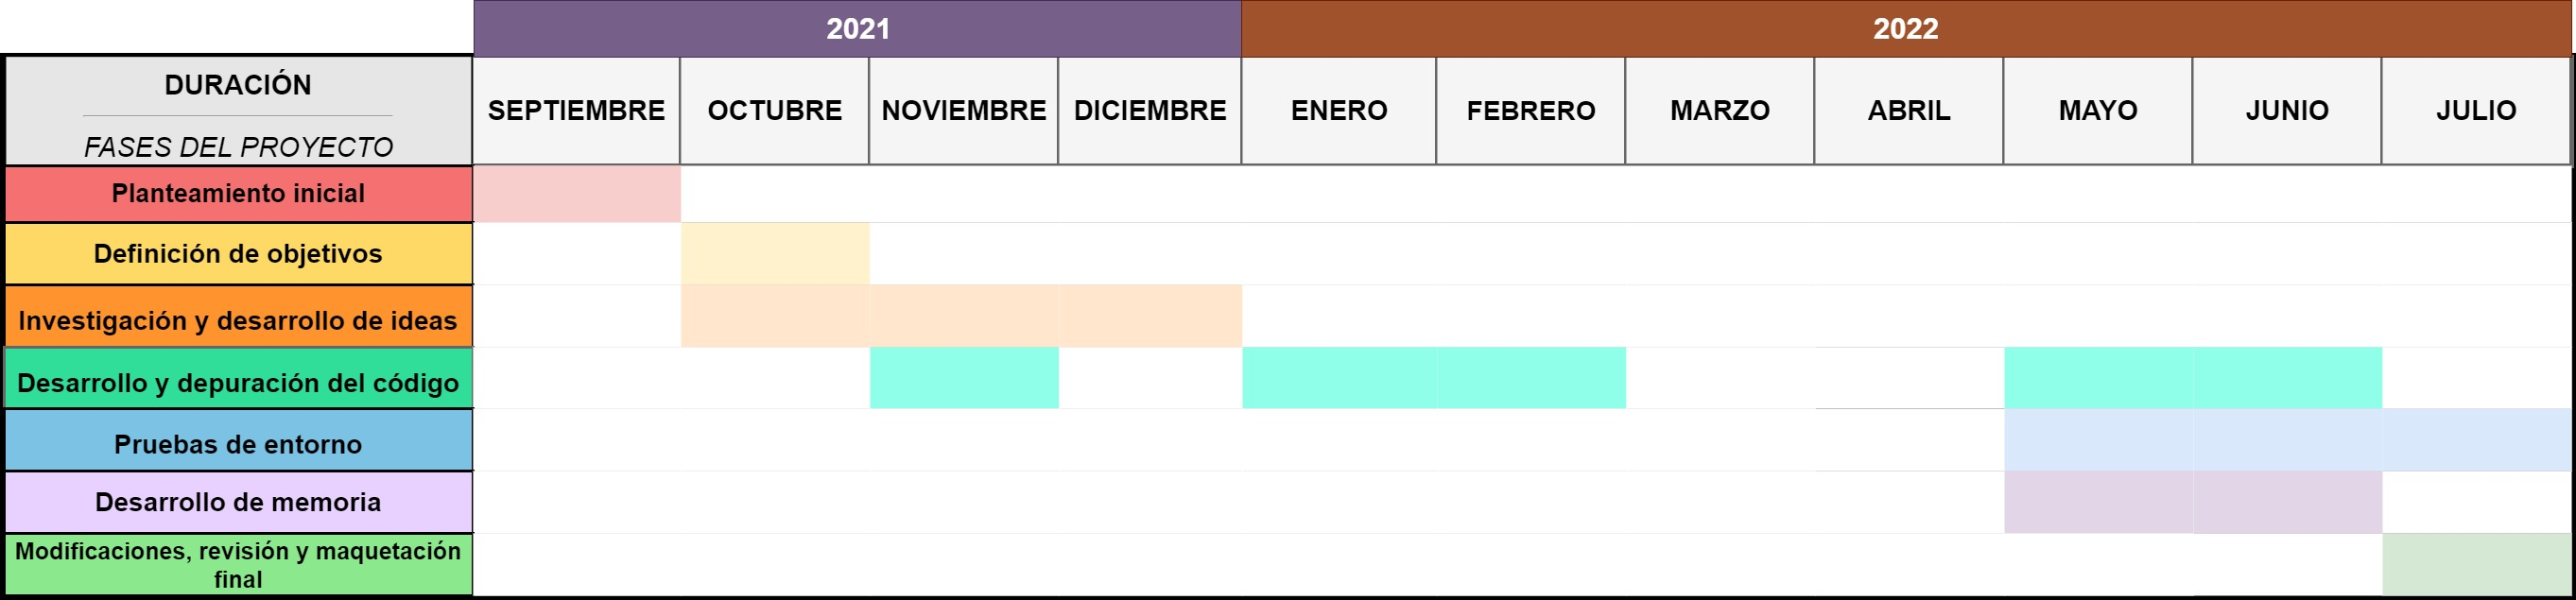
\includegraphics[width=17cm, keepaspectratio]{img/gantt.jpg}
    \caption{Diagrama de Gantt}
    \label{fig:diagrama_gantt}
\end{figure}

\pagebreak 
Para facilitar la organización, estructuración y consecución de objetivos se hace uso de la herramienta Trello\footnote{\url{https://trello.com/tfg_felipesandoval/boards}}, allí se dividen las tareas en tres bloques: \textbf{Investigativo} (Amarillo), \textbf{Desarrollo de código} (Verde) y \textbf{Desarrollo de memoria} (Rojo). En las imágenes \ref{fig:trello_corto}, \ref{fig:trello_medio} y \ref{fig:trello_largo} se pueden observar los distintos estados de los objetivos durante la elaboración del trabajo.

 \begin{figure}[h]
 	 \centering
    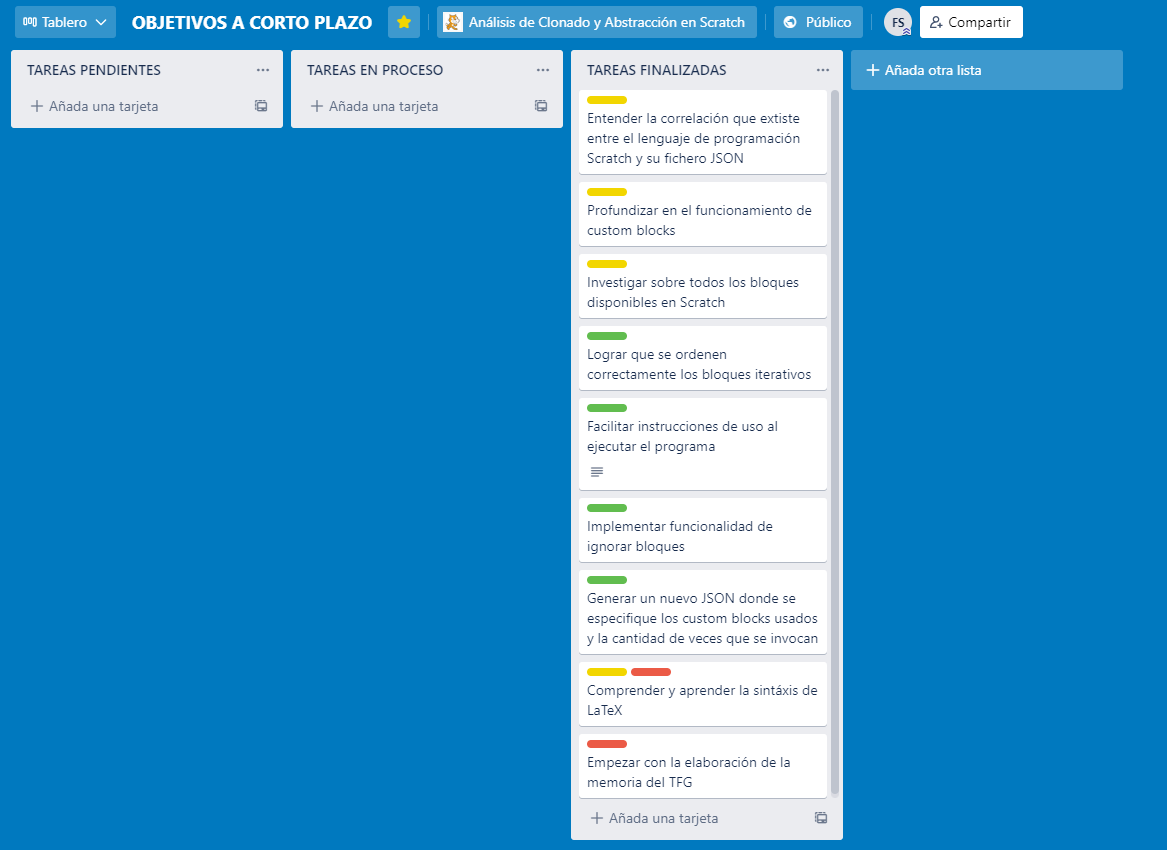
\includegraphics[width=15cm, keepaspectratio]{img/obj_cortoplazo.png}
    \caption{Tablero de Trello con objetivos a corto plazo}
    \label{fig:trello_corto}
 \end{figure}

 \begin{figure}[htb!]
  	 \centering
    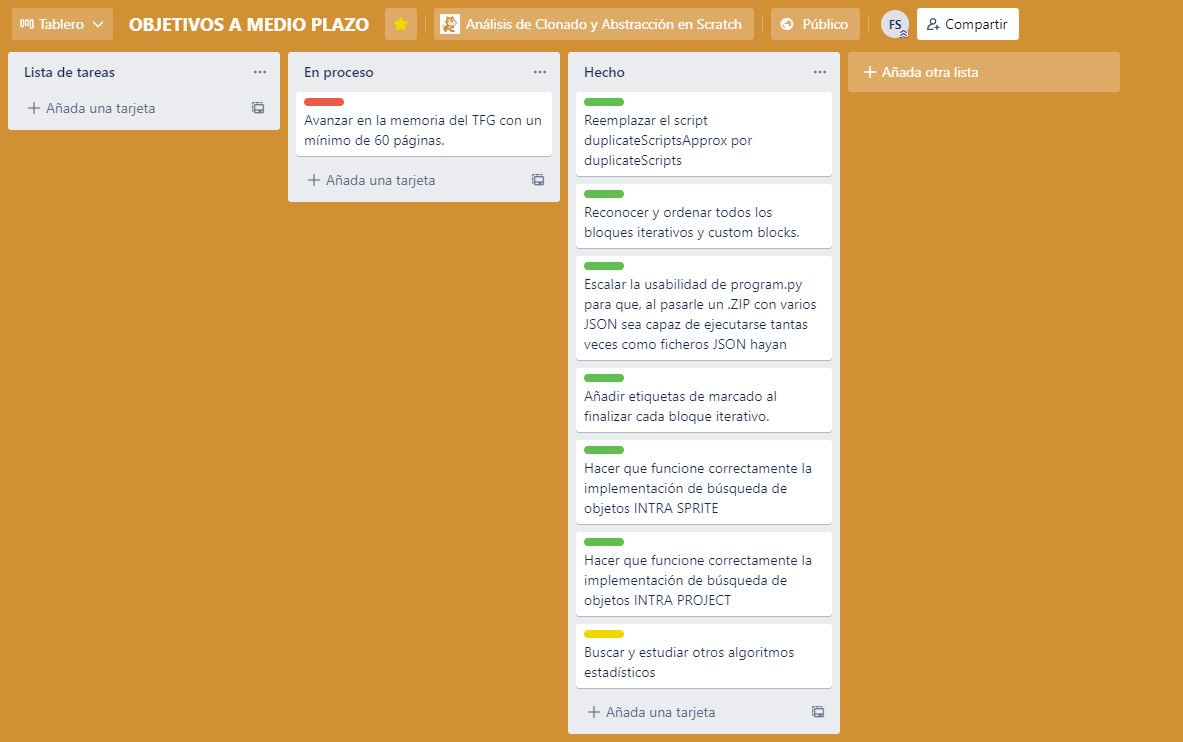
\includegraphics[width=17cm, keepaspectratio]{img/obj_medioplazo.png}
    \caption{Tablero de Trello con objetivos a medio plazo}
    \label{fig:trello_medio}
 \end{figure}
 
  \begin{figure}[htb!]
  	 \centering
    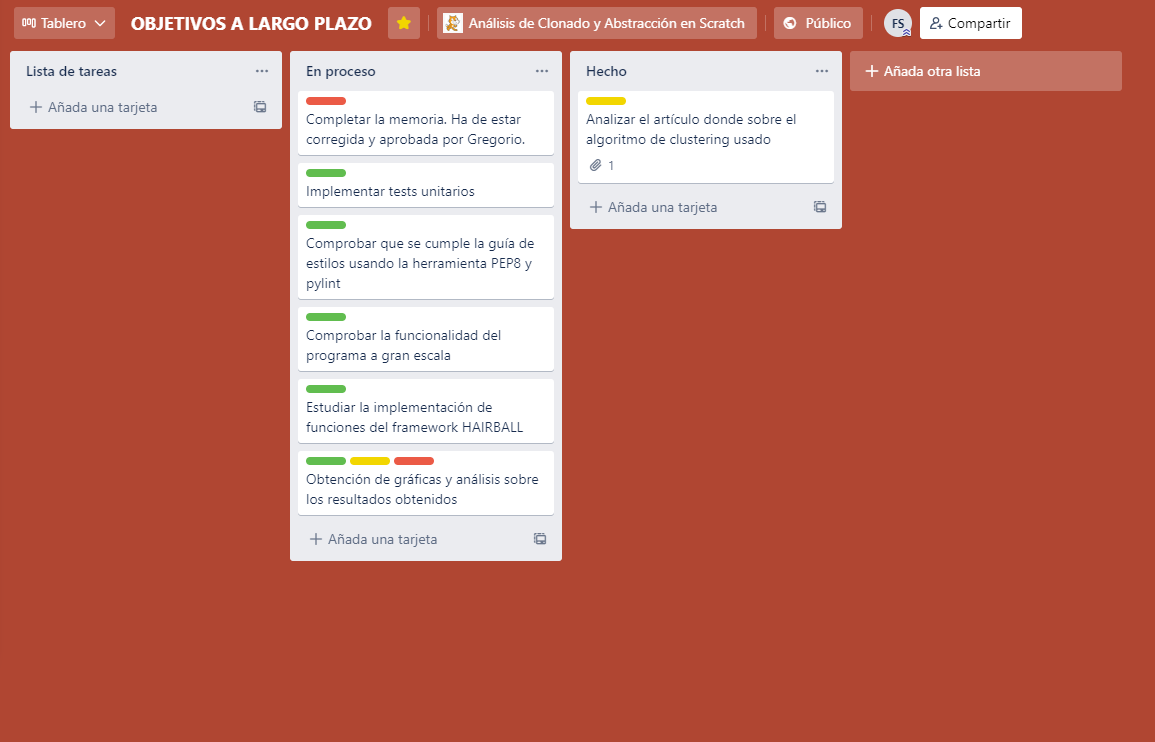
\includegraphics[width=17cm, keepaspectratio]{img/obj_largoplazo.png}
    \caption{Tablero de Trello con objetivos a largo plazo}
    \label{fig:trello_largo}
 \end{figure}
 
%A continuación, viene una figura, la Figura~\ref{figura:foro_hilos}. 
%También habrás tomado nota de cómo se ponen las ``comillas dobles'' para que se muestren correctamente. 
%Nota que hay unas comillas de inicio (``) y otras de cierre (''), y que son diferentes.
%Volviendo a las referencias, nota que al compilar, la primera vez se crea un diccionario con las referencias, y en la segunda compilación se ``rellenan'' estas referencias. 
%Por eso hay que compilar dos veces tu memoria.
%Si no, no se crearán las referencias.

%%%%%%%%%%%%%%%%%%%%%%%%%%%%%%%%%%%%%%%%%%%%%%%%%%%%%%%%%%%%%%%%%%%%%%%%%%%%%%%%
%%%%%%%%%%%%%%%%%%%%%%%%%%%%%%%%%%%%%%%%%%%%%%%%%%%%%%%%%%%%%%%%%%%%%%%%%%%%%%%%
% ESTADO DEL ARTE %
%%%%%%%%%%%%%%%%%%%%%%%%%%%%%%%%%%%%%%%%%%%%%%%%%%%%%%%%%%%%%%%%%%%%%%%%%%%%%%%%

\cleardoublepage
\chapter{Estado del arte}
\label{chap:estado}

En este capítulo se introducen las bases tecnológicas del trabajo.

\section{Scratch}
\label{sec:Scratch}

Scratch es un lenguaje de programación creado por el Grupo Lifelong Kindergarten del Laboratorio de Medios del MIT. En Scratch se permite programar historias interactivas, videojuegos, felicitaciones, animaciones, entre otros; todo esto a través de un entorno completamente visual que se fundamenta en el uso de personajes, escenarios y bloques gráficos que permiten la interacción entre ellos.

%FIXME: Aquí vendría bien una figura donde se vea Scratch

Entre sus cualidades desatacan que es totalmente gratuito, de uso libre, multilenguaje y altamente recomendado para la iniciación de niños y adolescentes en el mundo de la programación. Scratch es, además, una gran comunidad de usuarios de los que se puede aprender y compartir proyectos. Los mayores consumidores de Scratch en el mundo son Estados Unidos y Reino Unido, donde los niños que más lo usan son los que tienen una edad media entre los 13 y los 16 años.

Como se comentó previamente, en Scratch, los objetos se denominan \textit{sprites} y la parte visual es construida por piezas de puzle llamadas \textit{blocks} que al encajar entre sí forman funciones, conocidas como \textit{scripts}. En la imagen ~\ref{fig:scratch} se puede apreciar la pantalla principal de la interfaz gráfica de Scratch. Existen varias categorías de bloques, siendo de especial interés las siguientes: 

\begin{itemize}
  	\item \underline{Movimiento}: Usados para mover y girar un objeto por la pantalla.
  	\item \underline{Apariencia}: Usados para cambiar la visualización de un objeto.
  	\item \underline{Sonido}: Usados para reproducir o detener secuencias de audio.
  	\item \underline{Eventos}: Usados para controlar eventos que ejecuten determinadas acciones.
  	\item \underline{Datos}: Usados para para crear y asignar variables.
  	\item \underline{Control}: Usados para crear bucles o condicionales de ejecución.
  	\item \underline{Custom blocks}: Bloques definidos por el usuario. A modo de comparativa, son funciones personalizadas que podrán ser invocadas a lo largo del código.
\end{itemize}

\begin{figure}[htb!]
\centering
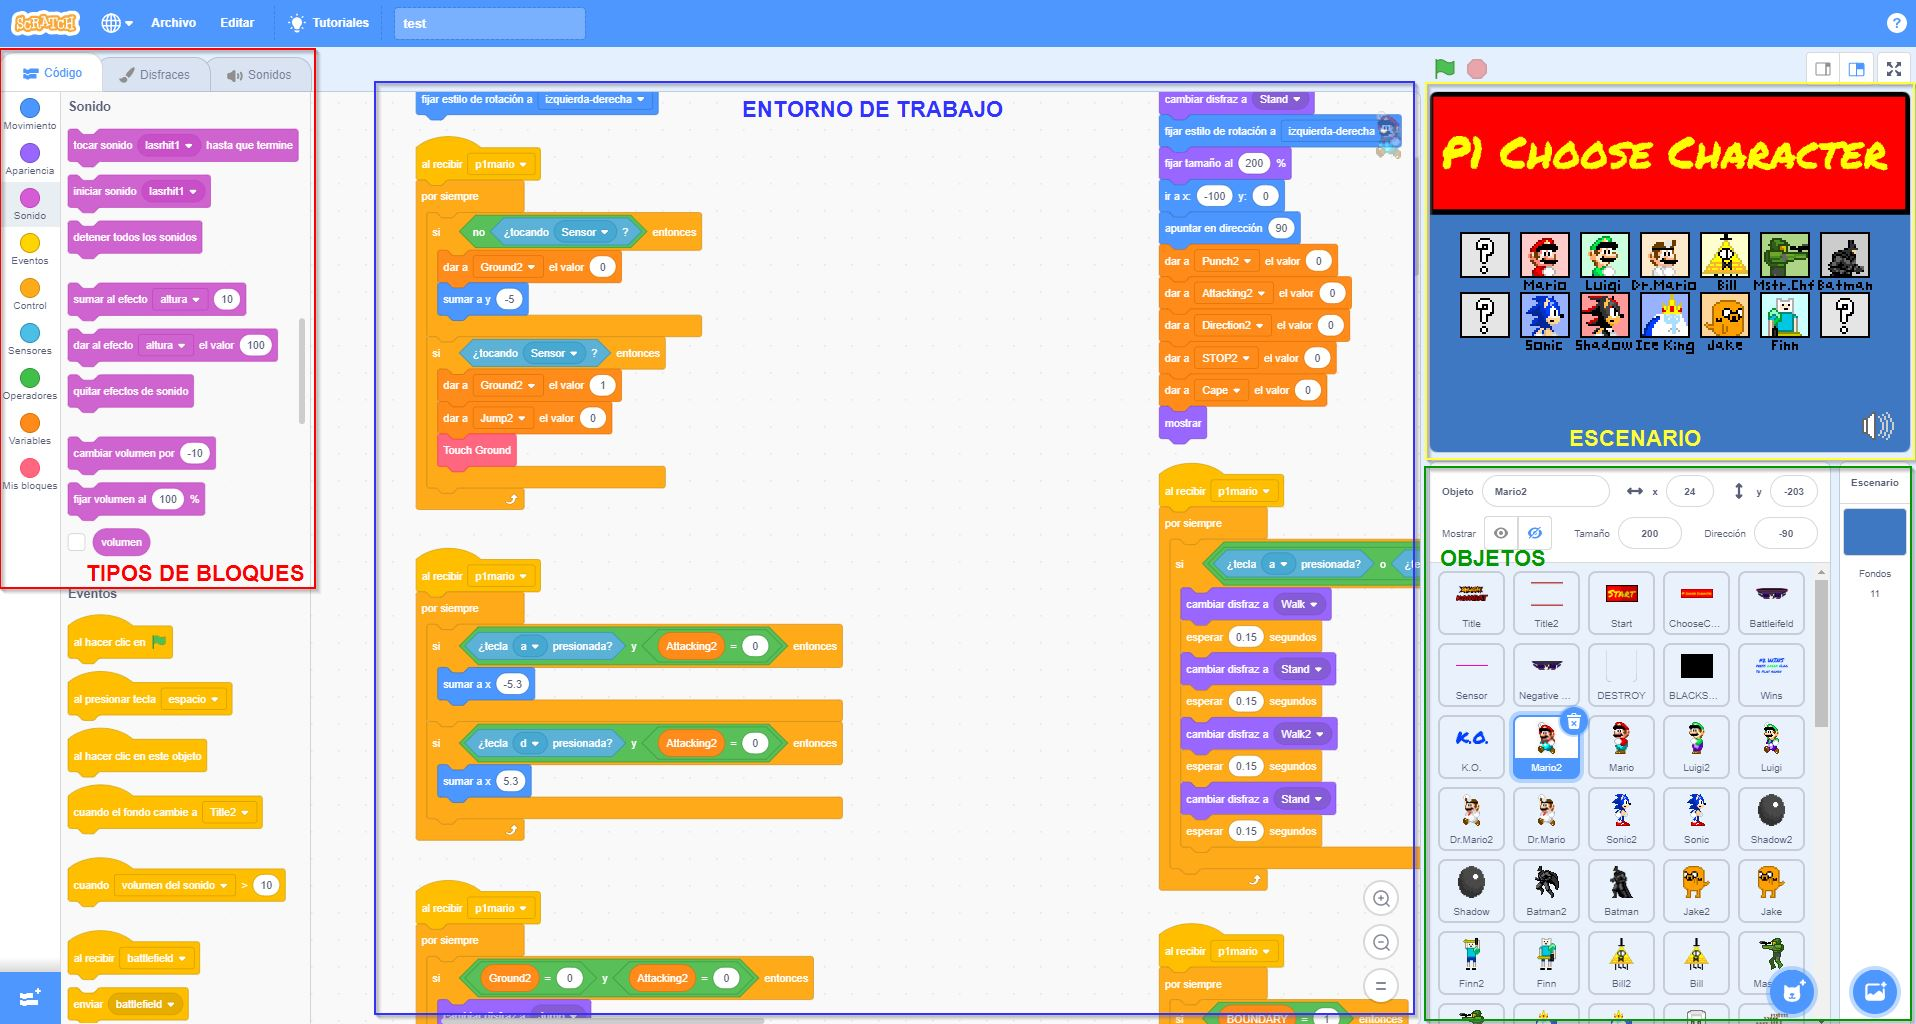
\includegraphics[width=17cm, keepaspectratio]{img/scratch.jpg}
\caption{Interfaz gráfica de Scratch}
\label{fig:scratch}
\end{figure}

La forma de programar en Scratch permite al usuario aprender rápidamente sin tener que comprender la sintaxis del lenguaje, centrándose en la lógica del programa, lo que mejora la habilidad de abstracción del usuario\cite{arotuma2017programacion}.

\section{JSON}
\label{sec:Json}

JavaScript Object Notation, mejor conocido como JSON, es un formato ligero de intercambio de datos que puede ser leído por cualquier persona. Este tipo de ficheros almacena información estructurada que es utilizada principalmente para transferir datos entre un servidor y un cliente\cite{jsonWeb}.

Teniendo en cuenta la sintaxis, existen dos elementos centrales en un fichero JSON \textit{Keys y Values}. Las \textit{Keys} o llaves contienen una secuencia de caracteres rodeados de comillas y los \textit{Values} o claves contienen un tipo de datos JSON válido, igualmente entre comillas. Puede tener la forma de un array, un diccionario, un string, un boolean, un objeto, un número o de tipo nulo. A modo ilustrativo, en el siguiente texto se puede apreciar un ejemplo de la estructura del formato JSON: %FIXME: aquí vendría bien una figura con un trozo de JSON (y que se explicara en el texto)

\begin{lstlisting}[language=json]
{
  "datos":{
    "objeto1": {
      "opcode": "loop",
      "blocks": [
        "bloque1", 
        "bloque2",
        "bloque3"
      ]
    },
    "objeto2": {
      "opcode": "custom",
      "blocks": [
        "customA", 
        "customB"
      ]
    }
  }
}
\end{lstlisting}

Es importante mencionar la estructura de un fichero JSON ya que es donde estará el código fuente de mi proyecto en Scratch.

\section{Python}
\label{sec:Python}

Es un lenguaje de programación interpretado cuya filosofía enfatiza el tener una sintaxis sencilla favorecedora al código legible. Se trata así de un lenguaje de programación multiparadigma, ya que soporta la programación orientada a objetos, la programación imperativa y la programación funcional~\cite{pythonWeb}. Python fue creado por Guido van Rossum a finales de los ochenta y su nombre se lo debe a los humoristas británicos \textit{`` Monty Python''}\footnote{https://platzi.com/blog/historia-python/}.

Existen tres versiones principales de Python pero las más extendidas son las versiones 2 y 3, siendo la versión 3.10 la última actualización disponible. En este proyecto se hace un uso íntegro de la versión Python 3.9. Cabe recalcar que las versiones 2 y 3 son incompatibles entre sí por el gran número de diferencias que existen entre ellas.

De todos los lenguajes de programación que aprendí a lo largo de la carrera he elegido Python por ser un lenguaje con una sintaxis sencilla, por ser multiplataforma, por su código abierto y, especialmente, por ser fuertemente tipado, ya que facilita la depuración de código y minimiza errores de compilación y ejecución.

Este proyecto se apoya en una serie de bibliotecas y módulos para Python. A continuación se enumeran y detallan el funcionamiento de cada uno:

\subsection{Sys}
\label{sec:sys}

Módulo que permite interactuar con parámetros y funciones específicas del sistema. Es usado para solicitar argumentos por consola y para detener la ejecución del programa mostrando un mensaje por pantalla. También es usado para registrar la información de los mensajes de error en el fichero de log de eventos.

\subsection{Os} 
\label{sec:os}

Módulo que permite trabajar, de forma portátil, con las funcionalidades del sistema operativo. En este proyecto se usa para eliminar ficheros JSON una vez han sido analizados, esto a fin de evitar crear excesivos documentos por cada ejecución.

\subsection{Shutil}
\label{sec:shutil}

Módulo que ofrece varias operaciones de alto nivel en archivos y colecciones de archivos. Es usado para copiar ficheros dentro de la ruta donde se ejecute el script.

\subsection{ZipFile}
\label{sec:zipfile}

Módulo que permite el manejo de archivos con extensión de tipo ZIP. Se usa para abrir, descomprimir y extraer ficheros dentro de este tipo de contenedores.

\subsection{JSON}
\label{sec:jsonmodule}

Módulo que ofrece la posibilidad de manipular ficheros de tipo JSON. Es usado para \textit{parsear}\footnote{Proceso de analizar una secuencia de símbolos a fin de determinar su estructura gramatical definida. También llamado análisis de sintaxis.} los elementos del fichero JSON de cada proyecto Scratch.

\subsection{Logging}
\label{sec:logging}

Módulo que define funciones y clases para implementar un registro de eventos de log para aplicaciones y bibliotecas. Se usa para generar el fichero \textbf{program\_logs.txt} que mostrará información relevante de la ejecución del programa. Es en este fichero donde se escribirán errores de ejecución y se detallará sobre la causa del fallo.

\subsection{Traceback}
\label{sec:traceback}

Módulo que copia el comportamiento del intérprete de Python cuando muestra una traza de pila. Es usado para obtener información de fallos relevantes en el fichero de logging.

\subsection{difflib}
\label{sec:difflib}

Módulo que implementa clases y funciones que ayudan a computar y trabajar con diferencias entre secuencias. Es especialmente útil para comparar texto e incluyen funciones que usan diversos algoritmos para lograr obtener esta información.

\subsubsection{SequenceMatcher}
\label{sec:difflib_SequenceMatcher} 

Clase flexible que se usa para comparar pares de secuencias de cualquier tipo, siempre y cuando los elementos de la secuencia sean separables. Esta clase implementa un método heurístico que identifica automáticamente ciertos elementos como no deseados, para ello cuenta cuantas veces aparece cada elemento en la secuencia. Se usa para comparar secuencias en cadenas de caracteres~\cite{sequenceWeb}.

\subsection{collections}
\label{sec:collections}

Este módulo implementa tipos de datos que proporcionan alternativas a los contenedores integrados de uso general de Python, como diccionarios, listas, sets, y tuplas~\cite{collectionWeb}.

\subsubsection{counter}
\label{sec:difflib_counter}

Es una subclase del tipo de datos \textit{dict} para contar objetos separables. Los elementos se almacenan como llaves y sus conteos se almacenan como valores de diccionario. Se permite que los conteos sean cualquier valor entero, incluidos los conteos a cero o negativos.

\subsubsection{defaultdict}
\label{sec:difflib_defaultdict}

Es una subclase del tipo de datos \textit{dict} que anula un método y añade una variable de instancia editable a través de una función para suministrar valores faltantes. Funciona de forma parecida a los diccionarios clásicos de Python.

\subsubsection{ordereddict}
\label{sec:difflib_ordereddict}

Es una subclase del tipo de datos \textit{dict} que tiene métodos especializados para reorganizar el orden del diccionario ya que recuerda las entradas en el orden que se agregaron.

\subsection{sklearn}
\label{sec:sklearn}

Este módulo es usado para ejecutar funciones y clases de Machine Learning construidas sobre SciPy~\cite{sklearnWeb}. Cuenta con algoritmos de clasificación, regresión, clustering y reducción de dimensionalidad. Además, es compatible con otras librerías de Python como NumPy y matplotlib.

\subsubsection{cluster}
\label{sec:sklearn_cluster}

Es una subclase que reúne diferentes algoritmos de agrupación no supervisada \textit{(unsupervised clustering)}. Dichos algoritmos ejecutan la tarea de agrupar conjunto de objetos con datos similares en grupos semejantes entre sí. Juega un papel primordial en el análisis de datos exploratorios y ofrece técnicas infalibles para el reconocimiento de patrones.

Aunque existen muchos algoritmos en esta subclase los más utilizados son K-medias y el algoritmo de propagación de afinidad \textbf{Affinity Propagation}, esto debido a su alta escalabilidad y tolerancia al ruido. En la imagen \ref{fig:comparativa_algoritmos} se pueden observar los clasificadores de distintos algoritmos incluidos en la subclase cluster. A efectos de este trabajo se describen los siguientes:

\begin{figure}[!htb]
    \centering
    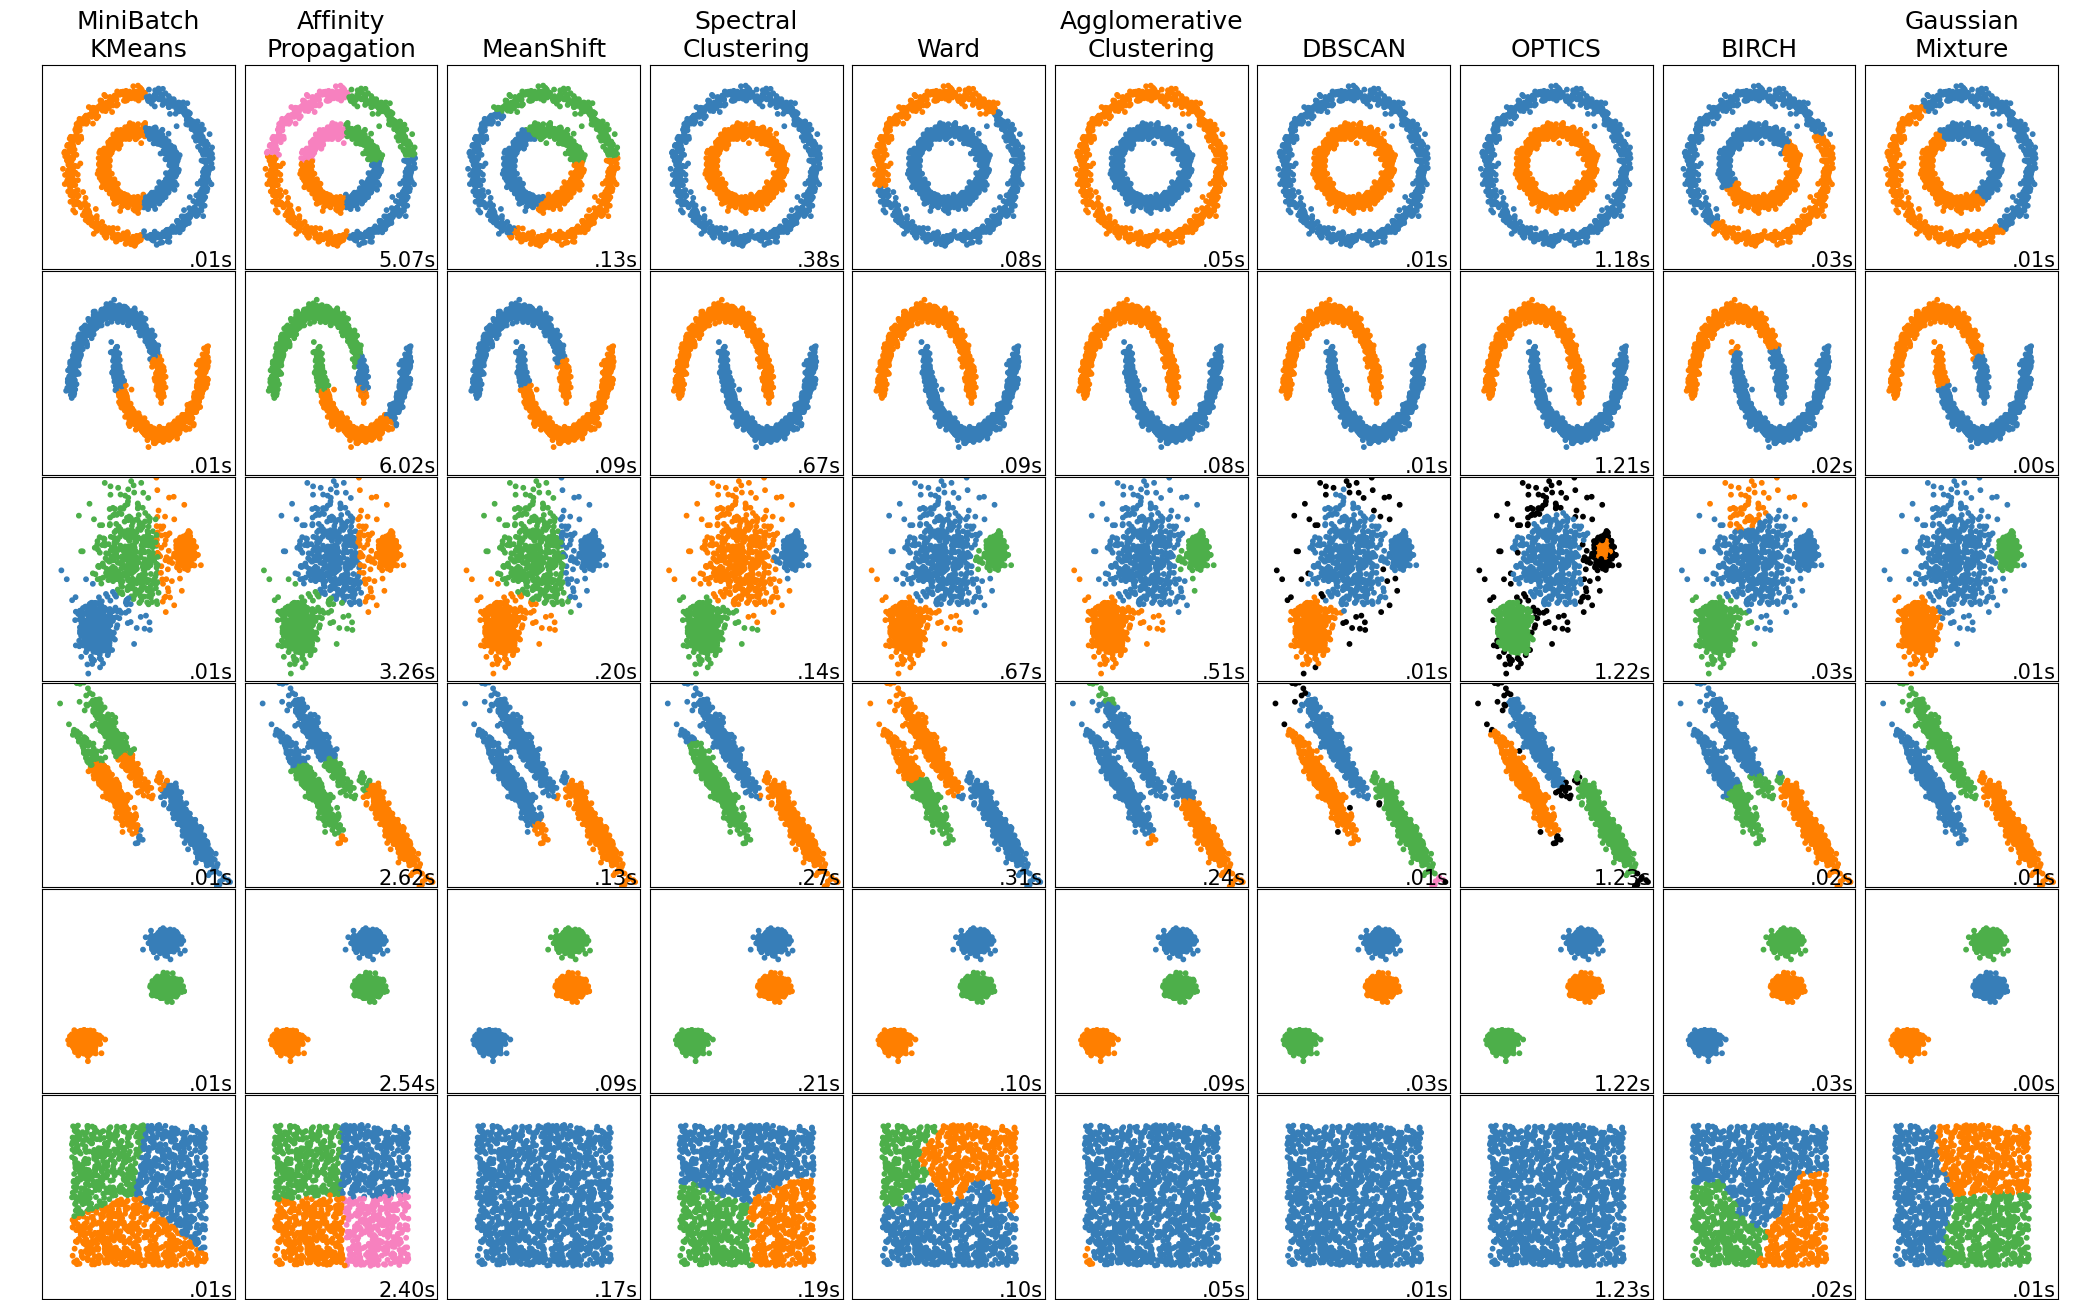
\includegraphics[width=17cm, keepaspectratio]{img/algorithm_comparison.png}
    \caption{Comparativa de algoritmos de clustering}
    \label{fig:comparativa_algoritmos}
\end{figure}

\begin{itemize}
\item \textit{Algoritmo de propagación por afinidad (Affinity Propagation)}: Se usa para encontrar grupos de objetos que son similares entre sí. El algoritmo toma como input un conjunto de objetos y un característica de similitud para devolver como output una lista de objetos que están agrupados por coincidencia. En la imagen \ref{fig:affinitypropagation} se puede apreciar un ejemplo del las iteraciones que realiza para clasificar el centro de los clústeres.
\item \textit{Algoritmo de K-medias (K-means)}: Se trata de un método de tipo divisivo, lo que significa que los datos se dividen en grupos más pequeños a medida que avanza el algoritmo. Su objetivo es asignar cada dato a un grupo de tal forma que los elementos dentro de un conjunto sean similares entre sí,  mientras que los datos de otros grupos sean lo más diferentes posible.
\end{itemize}

\begin{figure}[!htb]
    \centering
    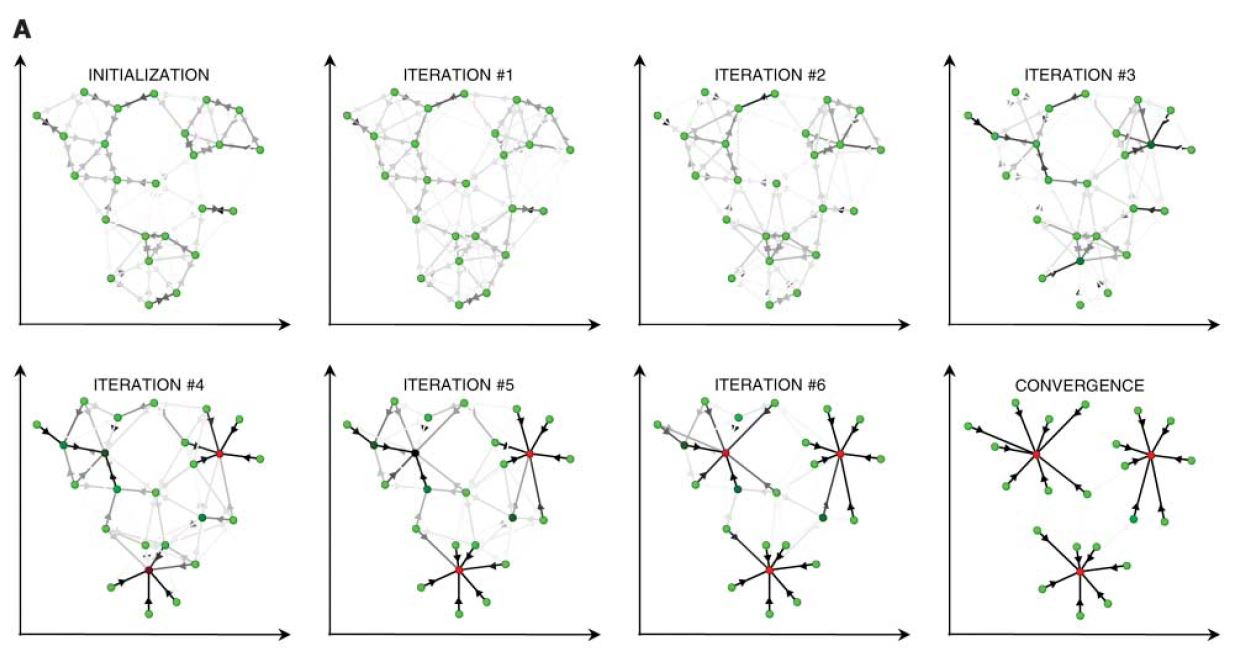
\includegraphics[width=16cm, keepaspectratio]{img/affinitypropagation.jpg}
    \caption{Funcionamiento ilustrativo del algoritmo de propagación por afinidad}
    \label{fig:affinitypropagation}
\end{figure}

En este trabajo se hará un uso exclusivo del algoritmo \textbf{Affinity Propagation} ya que, en teoría, es el más óptimo para la homogeneidad, integridad y similitud en conjuntos de cadenas de textos~\cite{areed2020python}.

%A mí me gustan las tablas.
%Mucho.
%Aquí un ejemplo de tabla, la Tabla~\ref{tabla:ejemplo} (siento ser pesado, pero nota cómo he puesto la referencia).

%\begin{table}
% \begin{center}
%  \begin{tabular}{ | l | c | r |} % tenemos tres colummnas, la primera alineada a la izquierda (l), la segunda al centro (c) y la tercera a la derecha (r). El | indica que entre las columnas habrá una línea separadora.
%    \hline
%    Uno & 2 & 3 \\ \hline % el hline nos da una línea vertical
%    Cuatro & 5 & 6 \\ \hline
%    Siete & 8 & 9 \\
%    \hline
%  \end{tabular}
%  \label{tabla:ejemplo}
%  \caption{Ejemplo de tabla. Aquí viene una pequeña descripción (el \emph{caption}) del contenido de la tabla. Si la tabla no es autoexplicativa, siempre viene bien aclararla aquí.}
% \end{center}
%\end{table}

\section{Hairball} 
\label{sec:Hairball}

Hairball en un plugin de Python que analiza proyectos de Scratch, ofreciendo a su salida información sobre el nivel de habilidades del pensamiento computacional, como abstracción, paralelismo, lógica, sincronización, control de flujo, interactividad con el usuario y representación de los datos.

El modulo hairball permite generar una representación gráfica sobre los datos de un proyecto Scratch. Esto es útil para visualizar el flujo de datos y el funcionamiento del programa. También otorga información sobre malos hábitos de programación cómo código duplicado, código muerto y mal nombramiento e inicialización de variables~\cite{boe2013hairball}.

\section{Pip} 
\label{sec:pip}

Pip es un gestor de paquetes para el ecosistema de Python que es capaz de instalar y administrar paquetes mediante línea de comandos~\cite{pipWeb}. Pip es el gestor con el que se han instalado todos los módulos y bibliotecas que no trae por defecto Python. Pip suele estar incluido al instalar Python, sin embargo, podría no ser así por lo que sería necesario su descarga.

\section{Unittest} 
\label{sec:unittest}

Unittest es una herramienta empleada para realizar tests en Python, tanto para clases y módulos enteros como para scripts. Creada por Kent Beck, permite la automatización de tests y la opción de crear colecciones. Además, no está ligada a ningún marco de reportes por lo que nos permite utilizar el mas conveniente~\cite{unittestWeb}. Para todo lo mencionado Unittest se sirve de tests fixtures, test cases, test suites y test runner, propios de la programación orientada a objetos, conceptos explicados a continuación. 

\begin{itemize}
	\item \textbf{Test fixture}: es la preparación del entorno de todas las características del test que queremos ejecutar.
	\item \textbf{Test case}: es la unidad individual del test, nos permite generar un test unitario para testear cada función.
	\item \textbf{Test suite}: es la colección de los test cases que se ejecutan y agrupan juntos, también puede existir una coleccion de test suites. Ejecutar una suite es lo mismo que ejecutar una serie de test cases individualmente.
	\item \textbf{Test runner}: es el componente encargado de ejecutar los tests y proporcionar un resultado. Puede disponer de una interfaz gráfica, texto o devolver un valor especial.
\end{itemize}
\newpage 
Para ejecutar el conjunto de test desarrollados en este proyecto es necesario ejecutar la siguiente orden en línea de comandos:

\begin{lstlisting}[style=consola,numbers=none]
$ python3 -m unittest discover
\end{lstlisting}

\section{Guía de estilo PEP8} 
\label{sec:pep8}

PEP8 (Python Enhancement Proposal 81) es una guía de estilos definida para Python. Se trata de un conjunto de recomendaciones cuyo objetivo es ayudar a escribir código de forma estándar y legible~\cite{pep8Web}. Es la guía de estilo elegida porque se usó durante la elaboración de prácticas en la asignatura Protocolos de Transmisión de Audio y Vídeos por Internet (PTAVI). Algunas de las reglas más importantes de esta guía son:

\begin{itemize}
	\item Indentación en cuatro espacios.
	\item Espacios antes de cada tabulación.
	\item Líneas limitadas a 79 caracteres.
	\item Saltos de línea con barra invertida.
\end{itemize}

Actualmente, la herramienta ha sido renombrada como \textbf{pycodestyle} y el comando de instalación necesario es el siguiente:

\begin{lstlisting}[style=consola,numbers=none]
$ pip install pycodestyle
\end{lstlisting}

%%%%%%%%%%%%%%%%%%%%%%%%%%%%%

%Hemos hablado de cómo incluir figuras.
%Pero no hemos dicho nada de tablas.
%A mí me gustan las tablas.
%Mucho.
%Aquí un ejemplo de tabla, la Tabla~\ref{tabla:ejemplo} (siento ser pesado, pero nota cómo he puesto la referencia).

%\begin{table}
% \begin{center}
%  \begin{tabular}{ | l | c | r |} % tenemos tres colummnas, la primera alineada a la izquierda (l), la segunda al centro (c) y la tercera a la derecha (r). El | indica que entre las columnas habrá una línea separadora.
%    \hline
%    Uno & 2 & 3 \\ \hline % el hline nos da una línea vertical
%    Cuatro & 5 & 6 \\ \hline
%    Siete & 8 & 9 \\
%    \hline
%  \end{tabular}
%  \label{tabla:ejemplo}
%  \caption{Ejemplo de tabla. Aquí viene una pequeña descripción (el \emph{caption}) del contenido de la tabla. Si la tabla no es autoexplicativa, siempre viene bien aclararla aquí.}
% \end{center}
%\end{table}

%%%%%%%%%%%%%%%%%%%%%%%%%%%%%%%%%%%%%%%%%%%%%%%%%%%%%%%%%%%%%%%%%%%%%%%%%%%%%%%%
%%%%%%%%%%%%%%%%%%%%%%%%%%%%%%%%%%%%%%%%%%%%%%%%%%%%%%%%%%%%%%%%%%%%%%%%%%%%%%%%
% DISEÑO E IMPLEMENTACIÓN %
%%%%%%%%%%%%%%%%%%%%%%%%%%%%%%%%%%%%%%%%%%%%%%%%%%%%%%%%%%%%%%%%%%%%%%%%%%%%%%%%

\cleardoublepage
\chapter{Diseño e implementación}

En este capítulo se realiza una descripción detallada de la estructura del software desarrollado y la funcionalidad a nivel de código. También se indica el hilo de ejecución, el entorno de trabajo y las herramientas usadas para la consecución de este proyecto.

\section{Entorno y herramientas de trabajo} 
\label{sec:entorno}

Para poder obtener resultados confiables en múltiples entornos, se compila, ejecuta y depura el código en los sistemas operativos Windows e UNIX. Se hace uso de tres aplicaciones para mantener sincronizados ficheros, historial de versiones y tener un control sobre la consecución de objetivos:

\begin{itemize}
  \item \textbf{Trello:} Aplicación usada para gestionar y organizar, a modo de tableros, las fases de las tareas a corto, medio y largo plazo. 
  \item \textbf{Dropbox:} Herramienta empleada como servicio de almacenamiento en la nube para mantener sincronizados ficheros, imágenes y referencias de la memoria.
  \item \textbf{GitHub:} Entorno usado para alojar el código y mantener un control de versiones. Resulta muy útil para dar marcha atrás en caso de errores o para crear nuevos hilos con modificaciones en el código.
\end{itemize}

En la imagen \ref{fig:diagrama_trabajo} se puede apreciar un diagrama del entorno y la comunicación entre las herramientas usadas.

 \begin{figure}[!h]
    \centering
    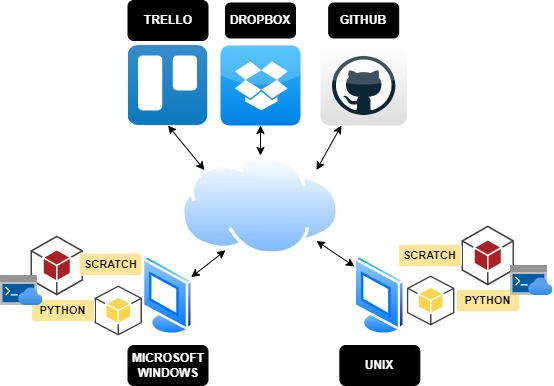
\includegraphics[width=9cm, keepaspectratio]{img/workplace.jpg}
    \caption{Diagrama de entorno y aplicaciones}
    \label{fig:diagrama_trabajo}
 \end{figure}

\section{Arquitectura general} 
\label{sec:arquitectura}

%Aquí viene todo lo que has hecho tú (tecnológicamente). Puedes entrar hasta el detalle.  Es la parte más importante de la memoria, porque describe lo que has hecho tú. Eso sí, normalmente aconsejo no poner código, sino diagramas.

%Si tu proyecto es un software, siempre es bueno poner la arquitectura (que es cómo se estructura tu programa a ``vista de pájaro'').

A nivel general, el flujo del funcionamiento del programa es el que se puede apreciar en la imagen \ref{fig:fasedesejecucion}. El script a ejecutar es \textit{program.py} y de allí se irán concatenando llamadas a \textit{duplicatescripts.py}, \textit{most\_frequent\_blocks.py}, \textit{statistics.py} y paralelamente, \textit{cluster.py}

\begin{figure}[!htb]
  \centering
  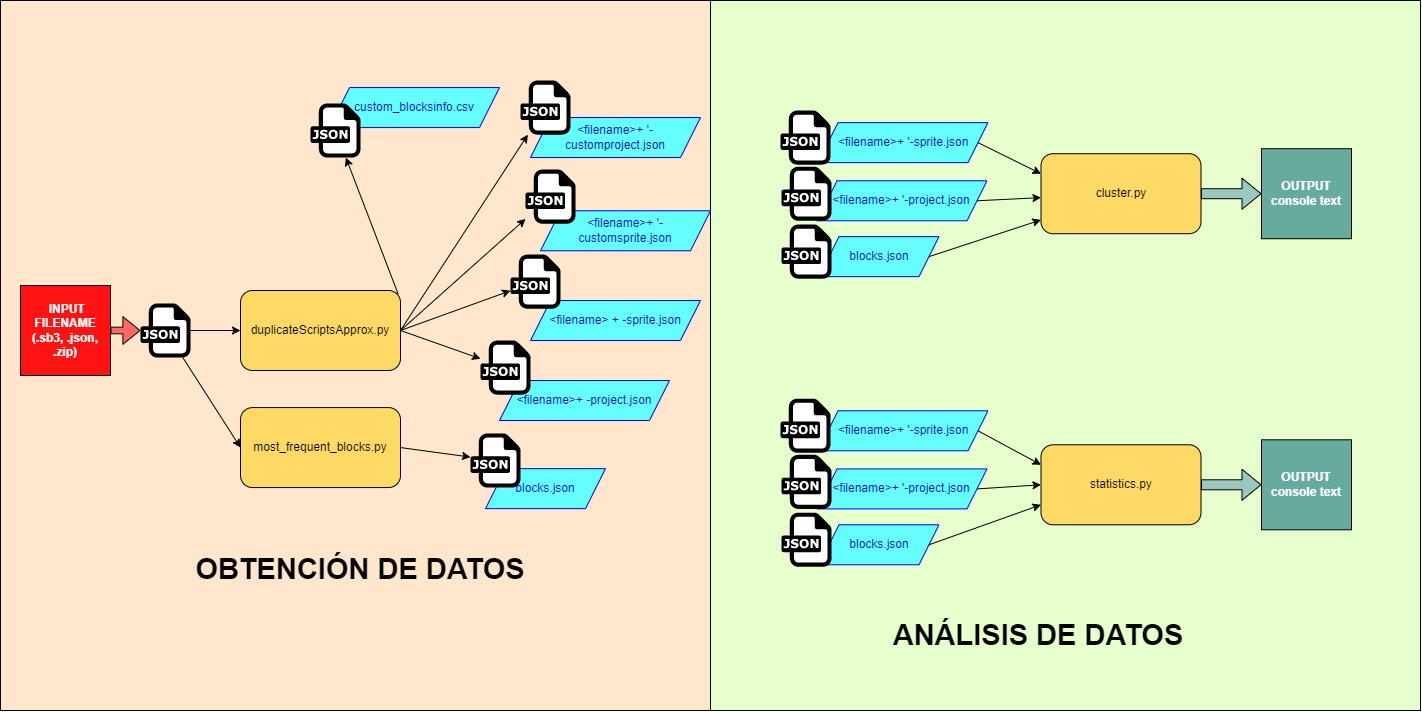
\includegraphics[width=17cm, keepaspectratio]{img/flow.jpg}
  \caption{Hilo de ejecución del programa}
  \label{fig:fasedesejecucion}
\end{figure}

Para ejecutar el software es necesario que el usuario pase por línea de comandos hasta un máximo de dos argumentos. Primero y obligatoriamente, el nombre del archivo a examinar, segundo y de forma opcional, el argumento \textbf{-i} que, de indicarlo, ignorará los bloques especificados en el fichero \textit{IgnoreBlocks.txt}. En caso de pasar más argumentos, el programa mostrará un mensaje de error y creará un fichero de registros en el que escribirá los eventos que ocurran durante la ejecución.

Los ficheros a analizar pueden estar en formato SB3 (extensión que emplea Scratch) en formato JSON o un fichero comprimido en formato ZIP. El software se ha desarrollado para ser escalable, por lo que, para realizar un análisis extensivo de muchos proyectos, es necesario comprimir los ficheros JSON en un contenedor ZIP. 

A continuación, se detallan los scripts, funciones y clases relevantes del software.

\subsection{program.py}

Sirve como script principal. Su tarea es controlar el hilo de ejecución de todo el programa, para ello extrae y recorre el contenido de ficheros JSON. Esto es posible a través de las funciones \textbf{sb3\_json\_extraction} y \textbf{obtaining\_json}. En este script se declara la forma como se escribirán los registros de control de ejecuciones en el archivo de logs, \textit{program\_logs.txt}. Este fichero resulta muy útil para depurar y encontrar excepciones durante la ejecución.

\subsection{duplicateScripts.py}

Este script toma como argumentos el nombre del fichero con su extensión correspondiente, el contenido del archivo JSON y el argumento opcional que indica si se ignoraran, o no, ciertos tipos de bloques.

El contenido del JSON se recorrerá como un de diccionario, empezando por la clave \textit{targets} que contiene todos los objetos. Seguidamente se extrae la información relevante de la clave \textit{blocks}, según el tipo de bloque que sea. En el código se irá almacenando en una variable de tipo diccionario, la clave/valor: \textit{block\_id:opcode}, la cual será importante para encontrar y añadir en su posición correcta a los bloques de control y \textit{custom blocks}. En la imagen \ref{fig:arboljson} se puede apreciar una vista de árbol generalizada sobre las clave/valor del fichero JSON, que según cada tipo de bloque contendrá más o menos información. 

Por otra parte, en la imagen \ref{fig:graljson} se puede apreciar un diagrama con la estructura general de un bloque genérico. Las claves de color amarillo siempre están presentes por lo que son importantes para organizar la estructura de mis bloques. Las claves de color verde no son importantes para la organización aunque aparezcan en todos los tipos de bloque. Las claves de color azul no siempre están presentes pero son igualmente importantes. Por último, las claves de color rojo no aparecen siempre y tampoco son relevantes.

\begin{figure}[!htb]
  \centering
  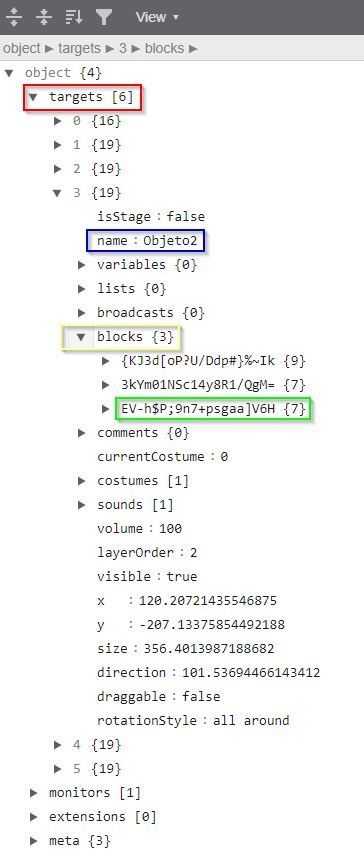
\includegraphics[width=7cm, keepaspectratio]{img/jsontree.jpg}
  \caption{Vista de árbol del contenido de un fichero JSON}
  \label{fig:arboljson}
\end{figure}

\begin{figure}[!htb]
  \centering
  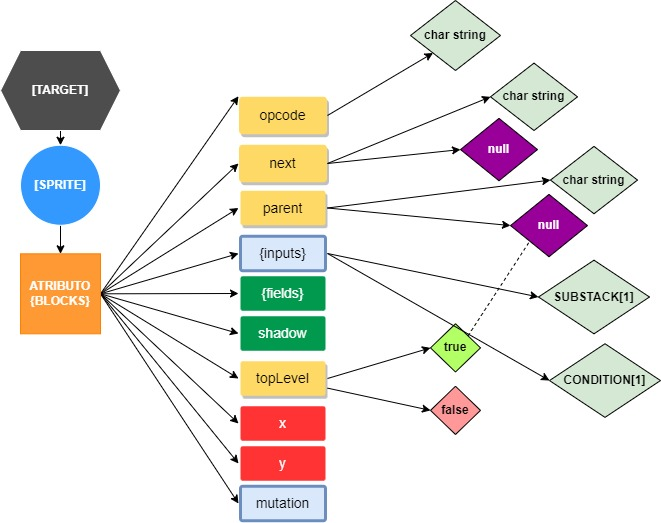
\includegraphics[width=13cm, keepaspectratio]{img/block_general.jpg}
  \caption{Estructura general de un bloque genérico}
  \label{fig:graljson}
\end{figure}

\newpage 
Como indicamos en el apartado anterior, todos los tipos de bloques suelen tener una estructura similar pero no todos sus campos son relevantes. Las claves como \textbf{opcode}, \textbf{parent}, \textbf{next} y \textbf{topLevel} son esenciales para la organización y extracción de datos. Otras claves, como \textbf{inputs} y \textbf{mutation} no aparecen en todos los tipos de bloques, sin embargo, son igualmente imprescindibles para obtener el orden correcto del conjunto de scripts. Es importante enfatizar que el \textit{Block\_ID} es un valor \textbf{único por bloque}, totalmente independiente del \textit{opcode}. A continuación, se enumeran los casos genéricos y particulares considerados:

\begin{enumerate}

\item Si el valor de \textbf{topLevel} es True significa que el elemento es el primer bloque de mi script. En este caso el valor de la clave \textbf{parent} es null. 

\item Si el valor de \textbf{topLevel} es False significa que el elemento no es el primer bloque. En este caso el valor de la clave \textbf{parent} contiene el \textit{Block\_ID} del bloque superior.

\item La clave de \textbf{opcode} siempre tendrá como valor un string con el nombre de ese bloque.


\item El valor de \textbf{next} puede ser un string con el \textit{Block\_ID} del siquiente bloque o puede ser null. En este último caso, puede ser porque es el último elemento del script, porque es un bloque de control \textit{(control\_repeat, control\_forever)} o porque es un bloque definido por el usuario \textit{(custom\_block)}. En la imagen \ref{fig:loopsforever} se puede apreciar un diagrama con las claves y valores relevantes para este tipo de bloques.

\item Dentro del valor \textbf{inputs} se encuentra otra clave llamada \textbf{substack} que contiene los elementos internos de los bloques de control (\textit{control\_repeat, control\_forever, control\_if, control\_repeat\_until y control\_if\_else)}. Este valor es exclúsivo de este tipo de bloques. En la imagen \ref{fig:controlblock} se ejemplifica este caso y en la imagen \ref{fig:scratch_control} se muestra la interfaz de Scratch, a modo de puzle, sobre el script y sus referencias en el JSON.

\item Para el caso especial del bloque \textit{control\_if\_else} el valor \textbf{substack2} contiene una lista con la secuencia de bloques internas en el hilo condicional. En la imagen \ref{fig:controlblock_spe} se ejemplifica la estructura especial de este tipo de bloques y en la imagen \ref{fig:scratch_special} se aprecia la interfaz de Scratch.

\item Se añaden las siguientes marcas de control al finalizar los siguientes bloques:
\begin{itemize}
\item Marca ``END\_IF'' al final de la primera condición de los bloques \textit{control\_if, control\_repeat\_until} y \textit{control\_if\_else}.
\item Marca ``END\_ELSE'' al final de la segunda condición del bloque \textit{control\_if\_else}.
\item Marca ``END\_LOOP'' al final de todos los bloques de control.
\end{itemize}
\end{enumerate}

\begin{figure}
  \centering
  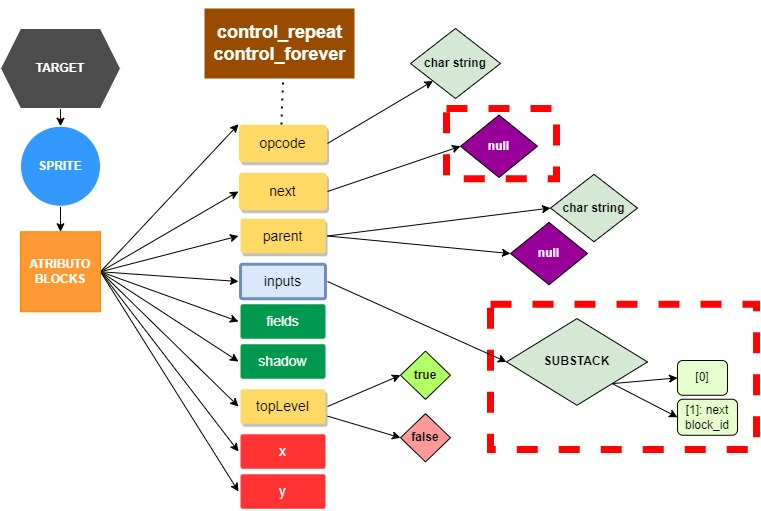
\includegraphics[width=15cm, keepaspectratio]{img/block_loop.jpg}
  \caption{Estructura general de un bloque de tipo control\_repeat o control\_forever}
  \label{fig:loopsforever}
\end{figure}

\begin{figure}
	\centering
  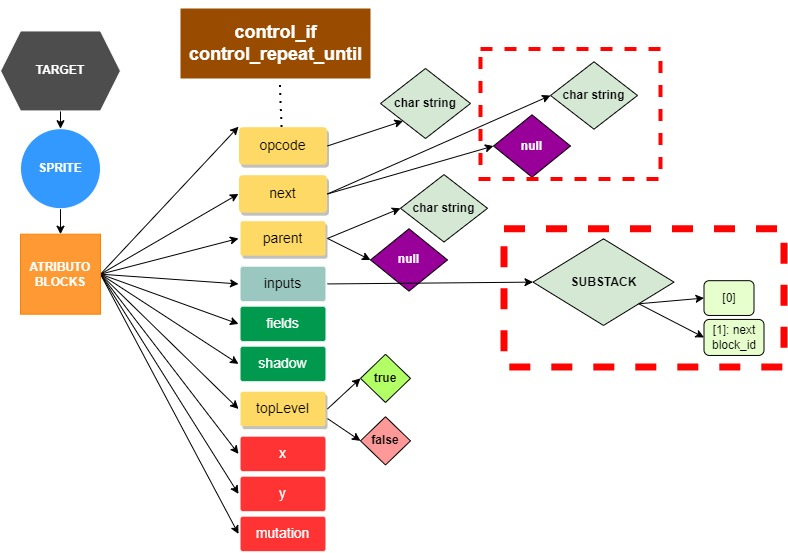
\includegraphics[width=15cm, keepaspectratio]{img/block_controlif.jpg}
  \caption{Estructura de un bloque condicional de tipo control\_if o control\_repeat\_until}
  \label{fig:controlblock}
\end{figure}

\begin{figure}
  \centering
  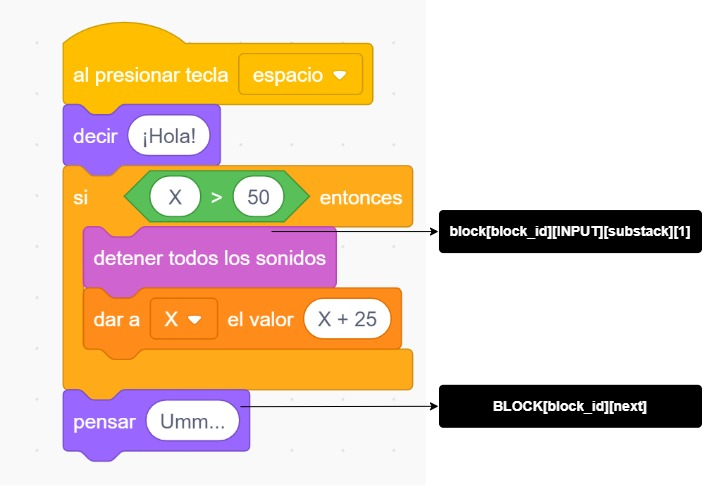
\includegraphics[width=13cm, keepaspectratio]{img/scratch_control.jpg}
  \caption{Script con bloque condicional de tipo control\_if}
  \label{fig:scratch_control}
\end{figure}

\begin{figure}
  \centering
  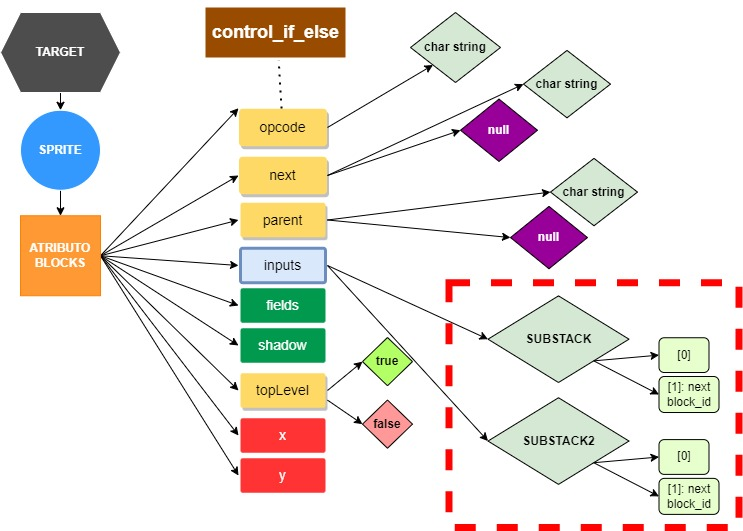
\includegraphics[width=15cm, keepaspectratio]{img/controlblock_spe.jpg}
  \caption{Estructura general de un bloque condicional de tipo control\_if\_else}
  \label{fig:controlblock_spe}
\end{figure}

\begin{figure}
  \centering
  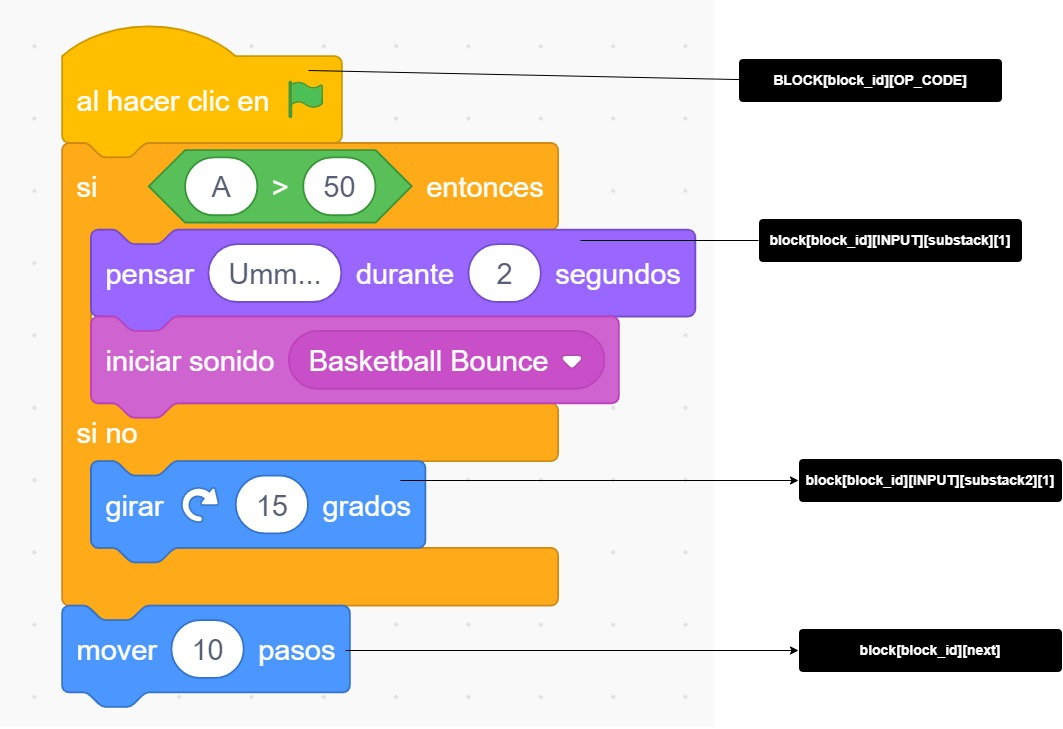
\includegraphics[width=13cm, keepaspectratio]{img/scratch_special.jpg}
  \caption{Script con bloque condicional de tipo control\_if\_else}
  \label{fig:scratch_special}
\end{figure}

\newpage 
Para los bloques personalizados por el usuario, los \textit{custom\_blocks}, se tienen en cuenta los tres siguientes casos:

\begin{enumerate}
\item Para elementos con \textbf{opcode} cuyo valor sea \textit{procedures\_prototype}:
\begin{itemize}
\item Su clave \textbf{next} tendrá siempre null como valor.
\item Su clave \textbf{parent} tiene como valor el block\_ID de \textit{procedures\_definition}.
\item Su clave \textbf{topLevel} tendrá siempre false como valor.
\item En su clave \textbf{mutation} se encuentra tanto el nombre de la función, como los argumentos y sus respectivos valores.
\end{itemize}

\item Para elementos con \textbf{opcode} cuyo valor sea \textit{procedures\_definition}:
\begin{itemize}
\item Su clave \textbf{parent} tendrá siempre null como valor.
\item Su clave \textbf{topLevel} tendrá siempre true como valor.
\item En su clave \textbf{inputs} se encuentra la sucesión de bloques que conforman mi custom block.
\end{itemize}

\item Para elementos con \textbf{opcode} cuyo valor sea \textit{procedures\_call}:
\begin{itemize}
\item En su clave \textbf{mutation} se encuentra el nombre de la función lo que permitirá contabilizar el número de llamadas.
\end{itemize}
\end{enumerate}

En las imágenes \ref{fig:block_prototype} y \ref{fig:block_definition} podemos apreciar un ejemplo sobre la estructura de las clave:valor que contiene el JSON. Por último, se realiza una comparación en la imagen \ref{fig:differences} sobre los distintos valores de cada bloque. Se aprecia que la información relevante para continuar con la organización secuencial está en \textit{procedures\_prototype} mientras que el contenido del custom block la tiene \textit{procedures\_definition}.

\begin{figure}[!htb]
  \centering
  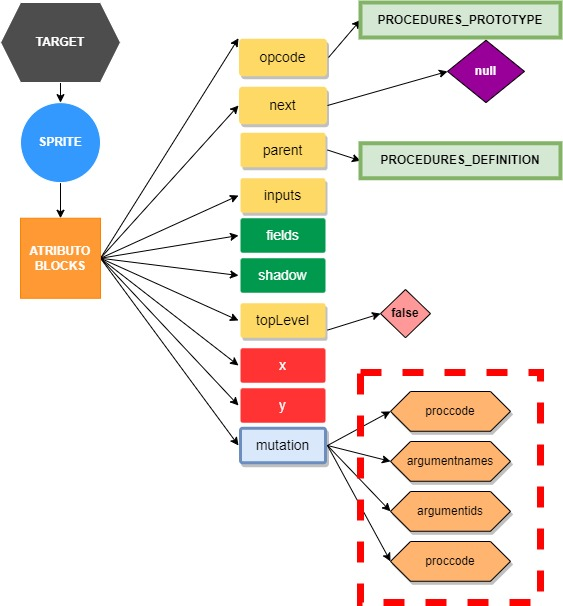
\includegraphics[width=10cm, keepaspectratio]{img/block_prototype.jpg}
  \caption{Estructura general de un bloque de tipo block\_prototype}
  \label{fig:block_prototype}
\end{figure}

\begin{figure}[!htb]
  \centering
  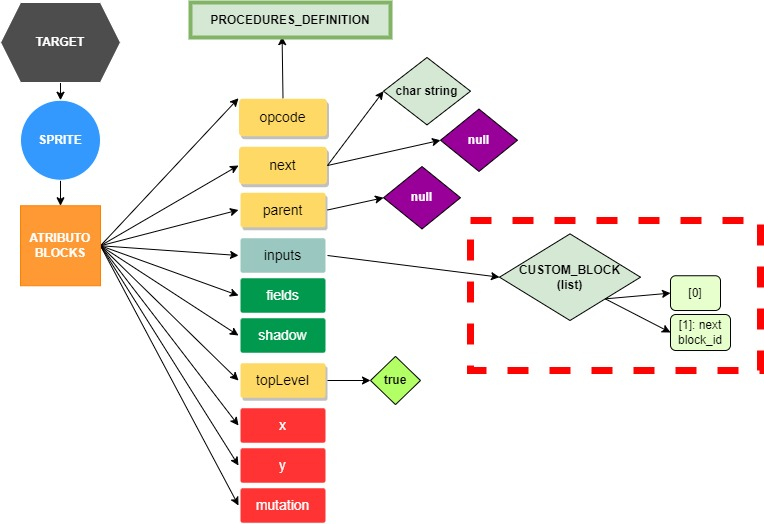
\includegraphics[width=13cm, keepaspectratio]{img/block_definition.jpg}
  \caption{Estructura general de un bloque de tipo block\_definition}
  \label{fig:block_definition}
\end{figure}

\begin{figure}[!htb]
  \centering
  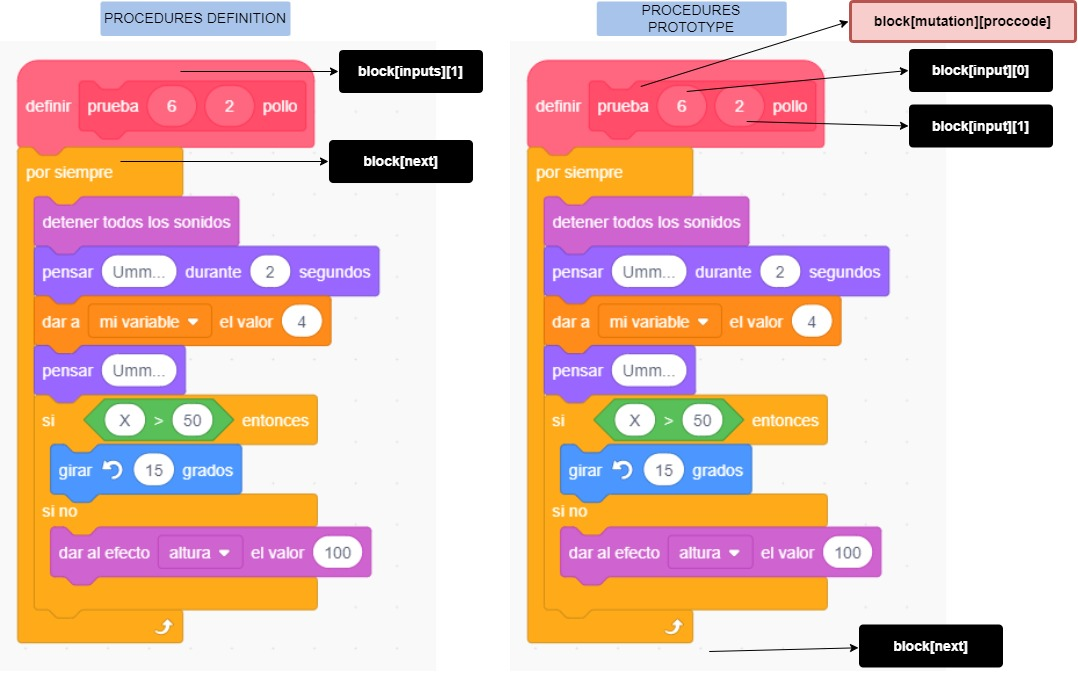
\includegraphics[width=14cm, keepaspectratio]{img/scratch_custom.jpg}
  \caption{Diferencias entre tipos de bloques custom\_block}
  \label{fig:differences}
\end{figure}

\newpage 
Uno de los principales problemas al momento de analizar el JSON ha sido ordenar de forma correcta la estructura de bloques, ya que por defecto no se muestran de forma ordenada. Para lograrlo se crean dos diccionarios: \textit{scripts\_dict} que almacena como valor los bloques de cada sprite y el diccionario \textit{blocks\_dict} que almacena como clave el block\_id de cada bloque y como valor su opcode. Además, este último es esencial para insertar bloques según el block\_id del parent que le corresponda.

Una vez se tiene todos los bloques de cada sprite ordenados se procede a obtener los bloques duplicados. Esto se logra gracias a la función \textbf{find\_dups}, que toma como argumento una lista de bloques. Puede ser, exclusiva para los bloques de cada objeto (\textit{intra-sprite})o para todos los bloques del proyecto (\textit{wide-project}). La función hace uso de la clase \textbf{sequenceMatcher} para comparar, palabra a palabra, cada bloque entre sí y devolver una lista con los bloque que más se repitan en cada iteración. 

% IMAGEN DE CODIGO, MEJOR NO.
%\begin{figure}
%  \centering
%  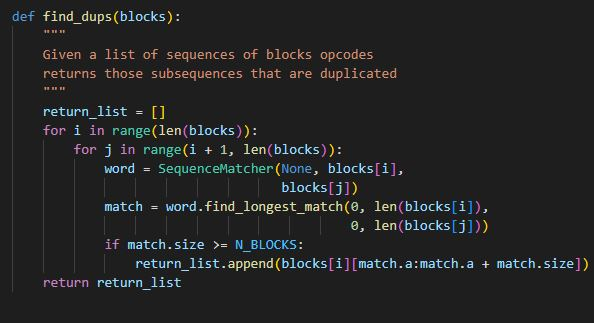
\includegraphics[width=13cm, keepaspectratio]{img/code_dups.jpg}
%  \caption{Código de la función find\_dups}
%  \label{fig:code_finddups}
%\end{figure}

\section{Obtención de datos} 
\label{sec:obtenciondatos}

Para finalizar \textbf{duplicateScripts.py}, se ejecuta la función \textbf{finalize} que genera tres ficheros de tipo JSON. En la imagen \ref{fig:flow_finddups} se puede apreciar un diagrama acerca esta última fase de ejecución.

\begin{itemize}
\item ``filename''-sprite.json: Contendrá las cadena de bloques mas repetidos por objeto.
\item ``filename''-project.json: Contendrá las cadena de bloques mas repetidos en todo el programa.
\item ``filename''-custom.json: Contendrá información relevante sobre los bloques personalizadoss presente en cada script, además del recuento de llamadas.
\end{itemize}

\begin{figure}[!htb]
  \centering
  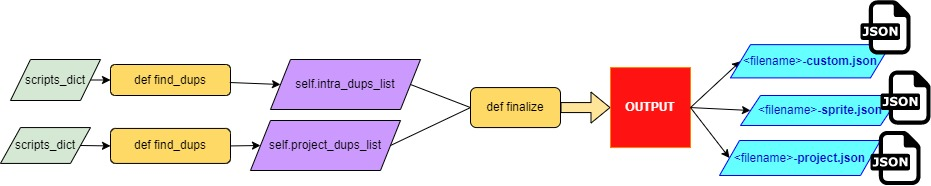
\includegraphics[width=17cm, keepaspectratio]{img/flow_duplicate.jpg}
  \caption{Diagrama de la última fase de ejecución duplicateScripts.py}
  \label{fig:flow_finddups}
\end{figure}

\subsection{most\_frequent\_blocks.py}

Este script toma como argumento un fichero JSON e itera sobre sus elementos para buscar y contabilizar los \textit{opcodes} de los bloques que más se repiten. Luego, ordena los bloques por frecuencia de uso y los guarda en un nuevo archivo JSON: \textbf{blocks.json} donde le asigna un caracter a cada bloque según su frecuencia de repetición. Al bloque mas repetido le corresponde la primera letra del abecedario y así sucesivamente completando la cadena de caracteres definida en la variable \textit{characters}. Se puede apreciar el diagrama del funcionamiento del script en la imagen \ref{fig:flow_mostfreq}.


%\begin{figure}
%  \centering
%  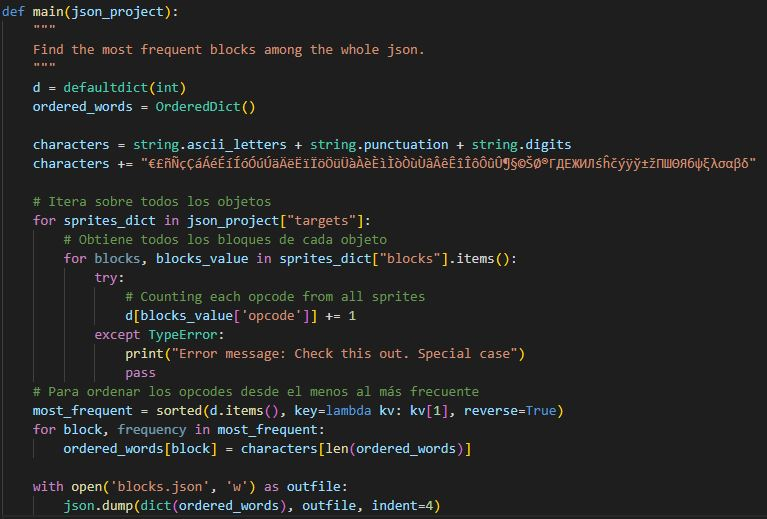
\includegraphics[width=13cm, keepaspectratio]{img/code_mostfrequent.jpg}
%  \caption{Código del script most\_frequent\_blocks.py}
%  \label{fig:code_mostfrequent}
%\end{figure}

\begin{figure}[!htb]
  \centering
  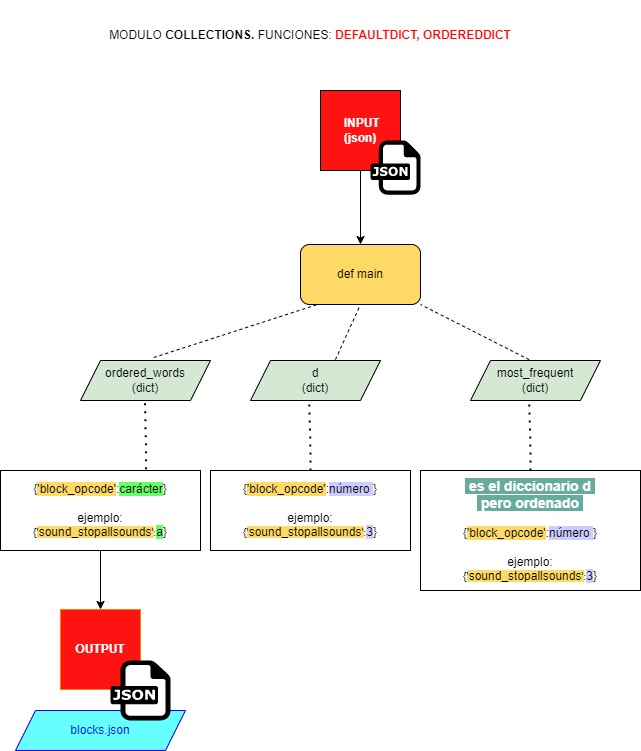
\includegraphics[width=14cm, keepaspectratio]{img/flow_mostfreq.jpg}
  \caption{Diagrama de funcionamiento de most\_frequent\_blocks.py}
  \label{fig:flow_mostfreq}
\end{figure}

\newpage 

\section{Procesado de datos} 
\label{sec:procesadodatos}

\subsection{statistics.py}

Este script analiza los ficheros JSON generados por el código de \textbf{duplicateScripts.py} con ayuda de los módulos \textit{counter}, \textit{defaultdict} y \textit{json}. Luego, la función \textbf{json2dna} carga el contenido del fichero \textbf{blocks.json} en el diccionario blocks\_dict y, a continuación, define la variable \textit{characters} que contiene todos los caracteres posibles. La función itera sobre cada elemento de la lista de duplicados y si el elemento no está en el diccionario del \textit{blocks.json}, se le asigna un nuevo caracter a dicho bloque. Luego, se añade al diccionario de scripts, cada secuencia de bloques con los caracteres correspondientes asignados en blocks\_dict.

Luego se añade el elemento al final de la lista block\_list. Finalmente, la lista block\_list se convierte en una cadena y se añade a la lista scripts. 

\begin{figure}[!htb]
  \centering
  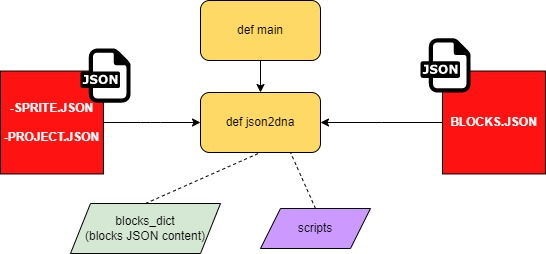
\includegraphics[width=13cm, keepaspectratio]{img/flow_statistics.jpg}
  \caption{Diagrama de funcionamiento de statistics.py}
  \label{fig:flow_statistics}
\end{figure}

\section{Análisis de datos} 
\label{sec:extracciondatos}

\subsection{cluster.py}

El algoritmo que se emplea es el algoritmo de propagación por afinidad es un algoritmo de aprendizaje automático que se utiliza para encontrar patrones ocultos en datos no estructurados. Se basa en la idea de que los datos que se parecen a unos pocos puntos de datos son más probable que sean similares a otros puntos de datos. El algoritmo se ejecuta en iteraciones, en cada iteración, se seleccionan algunos puntos de datos y se les asignan etiquetas. Luego, el algoritmo busca otros puntos de datos que se parezcan a los puntos de datos etiquetados y les asigna las mismas etiquetas. El algoritmo continúa iterando hasta que todos los puntos de datos hayan sido etiquetados.

El código de este script importa la función de levenshtein de la biblioteca distance y la función Counter de la biblioteca collections. Luego, define una función llamada json2dna que toma como argumento un archivo JSON y devuelve los scripts como caracteres. En la función main, el código convierte los scripts en una matriz y luego usa la función de levenshtein para calcular la similitud entre los scripts. Finalmente, el código imprime los resultados del clustering.

\section{Visualización de resultados} 
\label{sec:visualizacionresultados}

A continuación, un ejemplo genérico sobre como se visualizan los resultados por línea de comandos:

\begin{lstlisting}[style=consola,numbers=none]
*** STARTING ANALYSIS  ***

/// IGNORING BLOCKS ACTIVATED /// 
(se muestra solo si se pasa el argumento condicional -i)

-- STARTING DUPLICATESCRIPTS.PY SCRIPT --

Looking for duplicate blocks in (nombre de archivo)

Minimum number of blocks:  X

XX total blocks found
XX total blocks ignored
XX total scripts found
XX total sprites found
XX intra-sprite duplicate scripts found
XX project-wide duplicate scripts found
XX custom blocks found in all project
XX custom blocks calls found in all project

-- END OF DUPLICATESCRIPTS.PY SCRIPT --


-- GETTING INTRA SPRITE STATISTICS --

10 most common:
XX times
	BLOCK NAME 
	BLOCK NAME
	...

Different blocks: XX


-- GETTING INTRA PROJECT STATISTICS --

10 most common:
XXX times
	BLOCK NAME
	BLOCK NAME
	...


Different blocks: XX


-- STARTING CLUSTER.PY SCRIPT --

(CLUSTERING INFORMATION)

-- END OF CLUSTER.PY SCRIPT --


*** ENDING ANALYSIS  ***


\end{lstlisting}

%Recuerda que toda figura que añadas a tu memoria debe ser explicada.
%Sí, aunque te parezca evidente lo que se ve en la figura~\ref{fig:arquitectura}, la figura en sí solamente es un apoyo a tu texto.
%Así que explica lo que se ve en la figura, haciendo referencia a la misma tal y como ves aquí.
%Por ejemplo: En la figura~\ref{fig:arquitectura} se puede ver que la estructura del \emph{parser} básico, que consta de seis componentes diferentes: los datos se obtienen de la red, y según el tipo de dato, se pasará a un \emph{parser} específico y bla, bla, bla\ldots

%Si utilizas una base de datos, no te olvides de incluir también un diagrama de entidad-relación.


%%%%%%%%%%%%%%%%%%%%%%%%%%%%%%%%%%%%%%%%%%%%%%%%%%%%%%%%%%%%%%%%%%%%%%%%%%%%%%%%
%%%%%%%%%%%%%%%%%%%%%%%%%%%%%%%%%%%%%%%%%%%%%%%%%%%%%%%%%%%%%%%%%%%%%%%%%%%%%%%%
% EXPERIMENTOS, VALIDACIÓN Y RESULTADOS%
%%%%%%%%%%%%%%%%%%%%%%%%%%%%%%%%%%%%%%%%%%%%%%%%%%%%%%%%%%%%%%%%%%%%%%%%%%%%%%%%

\cleardoublepage
\chapter{Experimentos, validaciones y resultados}

%Este capítulo se introdujo como requisito en 2019. 
%Describe los experimentos y casos de test que tuviste que implementar para validar tus resultados. 
%Incluye también los resultados de validación que permiten afirmar que tus resultados son correctos. 

La experimentación para este proyecto se ha desarrollado a modo de ensayo y error. Primero, para probar la efectividad del código se crean muchos programas en Scratch, que de manera controlada contienen bloques de código duplicado con múltiples combinaciones a nivel \textit{intra-sprite} y \textit{wide-project}. Se ejecuta el programa varias veces y se evidencian las limitaciones al detectar estructuras complejas, imperfectos que poco a poco se va corrigiendo, hasta que los resultados coinciden con la información gráfica diseñada en Scratch. También se ejecuta la herramienta sobre un proyecto con multitud de objetos y bloques, el fichero \textbf{test.sb3} y se comprueba, al abrir el código en la interfaz de Scratch, que los resultados son verídicos.

Luego se decide poner a prueba la herramienta a gran escala. Para lograrlo se repite la ejecución iterativa en 200 ficheros (\textit{projects.zip}). Al terminar la primera ejecución se comprueban que hay ciertos JSON que no son posibles de analizar, estos quedan registrados en el fichero de errores \textbf{program\_logs.txt}. Se analizan uno a uno los ficheros problemáticos y se descubre que existen casos particulares en los que ciertas claves, consideradas imprescindibles para la estructuración y organización, no aparecen en algunos bloques. Finalmente se depuran los errores de detección con la ayuda de las pruebas unitarias tratando cada caso de forma general. Se confirma la robustez del software al obtener un resultado exitoso en todos los ficheros sin importar las múltiples combinaciones que pueda contener.

Para analizar la funcionalidad y robustez de mi código se crean los ficheros \textit{test\_program.py}, \textit{test\_DuplicateScripts.py} y \textit{test\_most\_frequent\_block.py} en los cuales se comprueba la salida de funciones y clases de manera controlada. Por ejemplo, en el fichero \textit{test\_DuplicateScripts.py} se crea un test case sobre la función \textbf{get\_custominfo}. Cuando en los datos de entrada están incompletos, bien sea porque falta un campo o porque está mal escrito, se observa que la salida no es la deseada. Esto se puede apreciar con la clave ``proccode'' que es requerida en esta función. También se confirma que si la clave no aparece en el diccionario Python muestra una excepción de error de tipo \textbf{KeyError}. En la imagen \ref{fig:code_testduplicate} se puede apreciar un extracto del código con las pruebas descritas.

\begin{figure}[!htb]
  \centering
  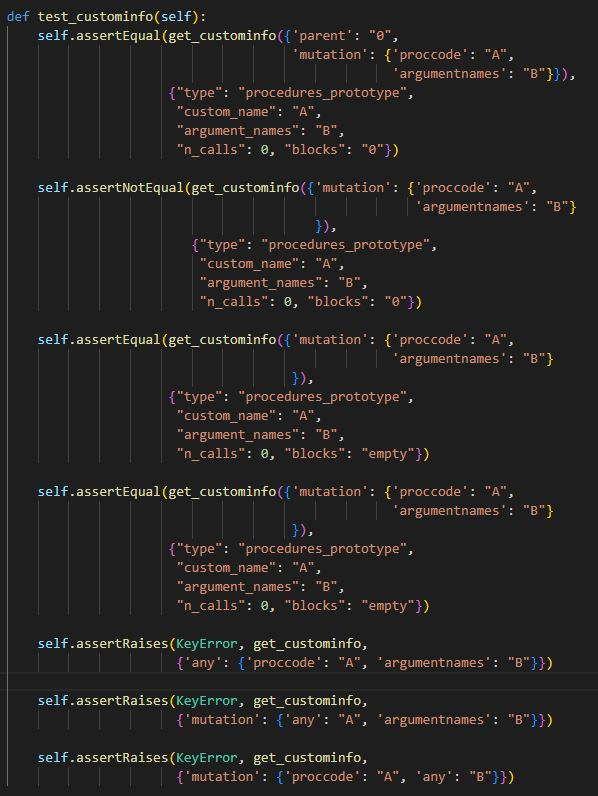
\includegraphics[width=13cm, keepaspectratio]{img/code_testduplicate.jpg}
  \caption{Código de un test case sobre una función de duplicateScripts.py}
  \label{fig:code_testduplicate}
\end{figure}

Para cuantificar el rendimiento
% FIXME: quizás aquí habría que hablar algo del rendimiento!  

%%%%%%%%%%%%%%%%%%%%%%%%%%%%%%%%%%%%%%%%%%%%%%%%%%%%%%%%%%%%%%%%%%%%%%%%%%%%%%%%
%%%%%%%%%%%%%%%%%%%%%%%%%%%%%%%%%%%%%%%%%%%%%%%%%%%%%%%%%%%%%%%%%%%%%%%%%%%%%%%%
% CONCLUSIONES %
%%%%%%%%%%%%%%%%%%%%%%%%%%%%%%%%%%%%%%%%%%%%%%%%%%%%%%%%%%%%%%%%%%%%%%%%%%%%%%%%

\cleardoublepage
\chapter{Conclusiones}
\label{chap:conclusiones}

Cuando empecé a aprender a programar en Scratch, una de las cosas que me llamó la atención fue la facilidad con la que se podía duplicar código. Al principio, no entendía realmente la importancia de esto, pero a medida que seguía aprendiendo más sobre este lenguaje, empecé a darme cuenta del impacto que esto tiene en el desarrollo de la abstracción. La razón por la que el código duplicado es un problema en Scratch es porque es un lenguaje de programación visual. Esto significa que el código no se escribe en texto sino que se crea encajando bloques, lo que facilita su copia y pega, bien sea intencionada o por accidente.

La abstracción es el proceso de ocultar complejidad detrás de una interfaz más simple. En Python, esto se consigue normalmente creando funciones o clases. Al abstraer los detalles de una parte concreta del código, hacemos que sea más fácil de entender y reutilizar. En Scratch, es un poco más complicado ya que la propia interfaz nos limita la reutilización de los bloques personalizados. Por ejemplo, si creamos una función elemental en el objeto \textit{``personaje''} solamente podremos hacer uso de ella dentro de dicho objeto obligando a crear nuevamente la función tantas veces como objetos se desee la implementen.

Por otro lado, el código duplicado es el que se repite varias veces en un programa. Esto puede ser un gran problema para la mantenibilidad porque si necesitamos cambiar el código, tendremos que cambiarlo en múltiples lugares u objetos en este caso. Esto puede conducir a errores si el código no se actualiza correctamente.

En la siguiente sección se debate sobre la consecución de los objetivos propuestos al inicio de este trabajo. 

\section{Consecución de objetivos}
\label{sec:consecucion-objetivos}

%Esta sección es la sección espejo de las dos primeras del capítulo de objetivos, donde se planteaba el objetivo general y se elaboraban los específicos.

%Es aquí donde hay que debatir qué se ha conseguido y qué no. 
%Cuando algo no se ha conseguido, se ha de justificar, en términos de qué problemas se han encontrado y qué medidas se han tomado para mitigar esos problemas.

%Y si has llegado hasta aquí, siempre es bueno pasarle el corrector ortográfico, que las erratas quedan fatal en la memoria final.
%Para eso, en Linux tenemos aspell, que se ejecuta de la siguiente manera desde la línea de \emph{shell}:

%\begin{verbatim}
%  aspell --lang=es_ES -c memoria.tex
%\end{verbatim}

El objetivo principal era crear una herramienta que fuera capaz de detectar la duplicidad de código en Scratch. Se puede concluir y confirmar que se logra dicho objetivo ya que se desarrolla una aplicación interactiva, a través de línea de comandos, capaz de contabilizar bloques, sprites, scripts e identificar aquellos que se repitan, tanto a nivel \textit{intra-sprite} como \textit{project-wide}. También se reconocen los \textit{custom blocks} y se contabilizan sus llamadas dentro del programa y, a la vez, se pueden omitir, según indicación del usuario, los bloques contenidos en el fichero \textit{IgnoreBlocks.txt}.

Toda la información sobre la duplicidad de código es mostrada a través de línea de comandos, de una forma legible y simplificada para que, con el código visual de Scratch, el usuario pueda hacer las correcciones pertinentes en su código redundante. 

Además es esto, se realizan pruebas con más de 200 archivos JSON contenidos en el fichero \textit{projects.zip}, los cuales son analizados, sin errores, informando sobre los bloques que mayor duplicidad presentan cada uno de los proyectos.

No existe una conclusión clara sobre la definición de patrones para detectar duplicidad de código, por lo menos no a nivel de programación. Esto se debe a que las pruebas han de realizarse con muchos mas proyectos, sin embargo, se propone su desarrollo en las futuras mejoras de los próximos trabajos.

Por último se realizan pruebas unitarias del código, esto garantiza que el funcionamiento y la ejecución de las funciones desarrolladas es el correcto según los valores que reciba.

\section{Conocimientos aplicados}
\label{sec:aplicacion}

%Aquí viene lo que has aprendido durante el Grado/Máster y que has aplicado en el TFG/TFM. Una buena idea es poner las asignaturas más relacionadas y comentar en un párrafo los conocimientos y habilidades puestos en práctica.

El aprendizaje y el conocimiento son fundamentales para el éxito en cualquier ámbito. A menudo, se asume que el conocimiento es una habilidad innata que se adquiere a través de la experiencia y el aprendizaje. Sin embargo, durante el transcurso del grado, me percate que para lograr el éxito se requiere de una combinación de capacitación, desarrollo del conocimiento y mucha práctica.

Quiero enumerar, por asignatura, las habilidades aprendidas que han facilitado la realización de este trabajo:

\begin{itemize}
\item \textbf{Informática I:} En esta asignatura tuve mi primer contacto con la programación. Aprendí las nociones básicas y aceleré el desarrollo de mi pensamiento computacional.
\item \textbf{Estadística para Sistemas Audiovisuales:} En esta asignatura aprendí como representar e interpretar datos. Ha sido de gran ayuda para analizar las gráficas de los experimentos realizados.
\item \textbf{Informática II:} En esta asignatura aprendí verdaderamente como programar. Aprendí un lenguaje complejo como Ada que me ayudó a organizar la legibilidad y eficiencia de mi código. 
\item \textbf{Protocolos para la Transmisión de Audio y Vídeo en Internet:} En esta asignatura comprendí realmente el alcance y las posibilidades del desarrollo de código. Fue mi primer contacto con Python, lo cual confirmó mi preferencia por las asignaturas en las que se tuviese que programar.
\item \textbf{Tratamiento Digital del Sonido y Tratamiento Digital de la Imagen:} En estas asignaturas descubrí como funcionan los algoritmos de clustering y sobre el Machine Learning. Fue realmente interesante descubrir estas técnicas para entender como determinar patrones y manejar grupos de datos.
\item \textbf{Construcción de Servicios y Aplicaciones Audiovisuales en Internet:} En esta asignatura aprendí sobre el desarrollo de aplicaciones web en lenguajes como HTML5, CSS, JavaScript, Node y Electron. Aunque en este proyecto no he tenido la oportunidad de desarrollar una interfaz web gráfica, me permitió reforzar mi interés en las asignaturas enfocadas en la programación, sin importar el lenguaje a usar.
\end{itemize}

\section{Conocimientos aprendidos}
\label{sec:aprendizaje}

El desarrollo de este trabajo ha supuesto un gran reto, pues es el primer proyecto que he realizado de esta complejidad. Durante las distintas etapas de elaboración he adquirido una serie de aprendizajes y habilidades que, a continuación, comparto:

\begin{itemize}
\item La importancia del desarrollo del pensamiento computacional. Al amar tanto la programación me he podido percatar que el pensamiento computacional es fundamental para el manejo de la información, la solución de problemas y la comprensión del comportamiento humano y debe desarrollarse preferentemente desde edades tempranas. Su desarrollo mejorará la competitividad e innovación, a la vez que forma nuevas aptitudes y valores en los niños~ \cite{wing_socialissues}.
\item La existencia de las pruebas unitarias, unittesting. De las lecciones que más me han marcado durante la realización de este proyecto, ya que su uso e implementación pasaran a ser fundamentales al momento de desarrollar software.
\item El lenguaje de programación Scratch. Desconocía totalmente la existencia de este lenguaje y su aplicación gráfica, de haberlo conocido seguro que hubiera desarrollado mi pasión por la programación a una edad más temprana. Considero alta su importancia para dar ese primer contacto con el mundo digital y para pensar de forma lógica a la vez que se resuelven problemas de forma creativa.
\item El uso de ficheros JSON y de archivos de log. He podido apreciar lo sumamente importante que es escribir y descifrar la información contenida en archivos JSON para entender la estructura de cualquier aplicación. También es importante la depuración de código a través de ficheros de control para así controlar y organizar los problemas que van surgiendo.  
\item Algoritmos de clustering en Python. He tenido la oportunidad de leer y aprender sobre diversos algoritmos, comparándolos entre sí y ampliando mi conocimiento sobre el alcances y utilidad que puede tener el aprendizaje máquina. 
\item La facilidad de \LaTeX. Aprender su estructura y semántica ha sido de gran utilidad para la maquetación de este trabajo.
\end{itemize}


\section{Trabajos futuros}
\label{sec:trabajos_futuros}

El software tiene un amplio rango de mejoras tanto a nivel de código como de funcionalidades. Se sugieren las siguiente implementaciones para los próximos trabajos:

\begin{itemize}
\item Brindar información al usuario donde se le indique otras alternativas para reducir la duplicidad de bloques, sin alterar la lógica del funcionamiento.
\item Mostrar gráficas, a modo informe, donde se muestren los bloques más duplicados basado en un estudio de múltiples proyectos.
\item Crear una interfaz gráfica para facilitar la interacción y uso. Se podría desarrollar una aplicación web interactiva alojada en GitLab.\footnote{https://about.gitlab.com/blog/2016/04/07/gitlab-pages-setup/}
\item Extender la funcionalidad de reconocimiento de bloques duplicados para reconocer la duplicidad de los \textit{custom blocks}, tanto a nivel \textit{intra-sprite} como \textit{project-wide}.
\item Integrar la herramienta en la aplicación de Dr. Scratch. Esto permitiría cuantificar a través de una puntuación la duplicidad de código presente.
\item Ampliar las conclusiones haciendo uso de una base de datos con infinidad de proyectos de Scratch.
\item Ampliar pruebas con otros algoritmos de clustering. Se podría realizar un trabajo investigativo donde se compare la efectividad entre algoritmos de aprendizaje supervizado y de aprendizaje no supervisado. Esto serviría para confirmar si efectivamente el algoritmo de propagación por afinidad es el más óptimo.
\end{itemize}


%Ningún proyecto ni software se termina, así que aquí vienen ideas y funcionalidades que estaría bien tener implementadas en el futuro.

%Es un apartado que sirve para dar ideas de cara a futuros TFGs/TFMs.

%%%%%%%%%%%%%%%%%%%%%%%%%%%%%%%%%%%%%%%%%%%%%%%%%%%%%%%%%%%%%%%%%%%%%%%%%%%%%%%%
%%%%%%%%%%%%%%%%%%%%%%%%%%%%%%%%%%%%%%%%%%%%%%%%%%%%%%%%%%%%%%%%%%%%%%%%%%%%%%%%
% BIBLIOGRAFIA %
%%%%%%%%%%%%%%%%%%%%%%%%%%%%%%%%%%%%%%%%%%%%%%%%%%%%%%%%%%%%%%%%%%%%%%%%%%%%%%%%

\cleardoublepage

% Las siguientes dos instrucciones es todo lo que necesitas
% para incluir las citas en la memoria
\bibliographystyle{ieeetr}
\bibliography{memoria}
% memoria.bib es el nombre del fichero que contiene
% las referencias bibliográficas. Abre ese fichero y mira el formato que tiene,
% que se conoce como BibTeX. Hay muchos sitios que exportan referencias en
% formato BibTeX. Prueba a buscar en http://scholar.google.com por referencias
% y verás que lo puedes hacer de manera sencilla.
% Más información: 
% http://texblog.org/2014/04/22/using-google-scholar-to-download-bibtex-citations/

%%%%%%%%%%%%%%%%%%%%%%%%%%%%%%%%%%%%%%%%%%%%%%%%%%%%%%%%%%%%%%%%%%%%%%%%%%%%%%%%
%%%%%%%%%%%%%%%%%%%%%%%%%%%%%%%%%%%%%%%%%%%%%%%%%%%%%%%%%%%%%%%%%%%%%%%%%%%%%%%%
% APÉNDICE(S) %
%%%%%%%%%%%%%%%%%%%%%%%%%%%%%%%%%%%%%%%%%%%%%%%%%%%%%%%%%%%%%%%%%%%%%%%%%%%%%%%%

\cleardoublepage
\appendix

\chapter{Manual de uso}
\label{app:manual}

%Esto es un apéndice.
%Si has creado una aplicación, siempre viene bien tener un manual de usuario.
%Pues ponlo aquí.

\subsection{Descarga de ficheros}
El código del trabajo desarrollado se puede encontrar alojado en el siguiente repositorio de GitHub: \textbf{https://github.com/felipsandoval/duplicatescripts-scratch}

\subsection{Requisitos}

Para poder hacer uso del programa es necesario tener instalado una serie de módulos y bibliotecas de Python. Para instalar todas estas dependencias es necesario ejecutar el siguiente comando:

\begin{lstlisting}[style=consola,numbers=none]
$ pip install -r requirements.txt
\end{lstlisting}

\subsection{Unittest}

Para ejecutar el conjunto de test y verificar que las funciones, módulos y clases funcionan correctamente, es necesario ejecutar la siguiente orden por línea de comandos:

\begin{lstlisting}[style=consola,numbers=none]
$ python3 -m unittest discover
\end{lstlisting}

\newpage 

\subsection{Uso}

\begin{lstlisting}[style=consola,numbers=none]
$ python3  program.py  <fichero(.SB3 o .JSON o .ZIP)>  [-i]
\end{lstlisting}

-i \textit{(OPCIONAL)}: Ignora los valores de bloques especificados en IgnoreBlocks.txt. También se ignoran las marcas de control: \textbf{END\_LOOP}, \textbf{END\_IF} y \textbf{END\_ELSE\_IF}.

\end{document}